% =====================================================================
%  TFM - Master en Machine Learning for Health (UC3M)
%  Portada oficial UC3M + cuerpo en formato IEEE (IEEEtran, 2 columnas)
%  Bibliografia con BibTeX -> referencias.bib
%
%  WORK IN PROGRESS: introduccion cerrada por Miguel + borrador de
%  Materiales y Metodos y Resultados pendiente de revision.
% =====================================================================
\documentclass[10pt,conference]{IEEEtran}

% --- Idioma, codificacion y matematicas -----------------------------
\usepackage[utf8]{inputenc}
\usepackage[T1]{fontenc}
\usepackage[english]{babel}
\usepackage{amsmath,amssymb,amsfonts}

% --- Graficos, color y tablas ---------------------------------------
\usepackage{graphicx,float,subcaption}
\usepackage[table]{xcolor}
\usepackage{booktabs,multirow,tabularx}
\graphicspath{{imagenes/}}
\definecolor{azulUC3M}{RGB}{0,0,102}

% --- Unidades y algoritmos ------------------------------------------
\usepackage{siunitx}
\sisetup{detect-all, range-units=single,
         separate-uncertainty=true, per-mode=symbol}
\usepackage{algorithm,algpseudocode}

% --- Numeracion: arabigos en vez de los romanos de IEEEtran ---------
% Por defecto IEEEtran da  I. / B. / 3)  y aqui se quiere  2 / 2.1 / 2.1.1
%
% OJO: no basta con redefinir \thesection y compania. Esas mandan en las
% referencias cruzadas, pero para los TITULOS la clase usa unas macros
% propias terminadas en "dis" (de display), definidas en IEEEtran.cls
% alrededor de la linea 2585 y usadas por \@seccntformat. Si solo se
% cambian las primeras, los \ref salen bien y los encabezados siguen en
% romanos y letras, que es justo lo que pasaba.
\renewcommand{\thesection}{\arabic{section}}
\renewcommand{\thesubsection}{\thesection.\arabic{subsection}}
\renewcommand{\thesubsubsection}{\thesubsection.\arabic{subsubsection}}
\makeatletter
\def\thesectiondis{\thesection}
\def\thesubsectiondis{\thesubsection}
\def\thesubsubsectiondis{\thesubsubsection}
\makeatother
% Tablas: IEEEtran las numera en romanos (TABLE I). Figuras ya van en
% arabigos, pero se fija tambien para que no dependa de la clase.
\renewcommand{\thetable}{\arabic{table}}
\renewcommand{\thefigure}{\arabic{figure}}

% --- Citas IEEE + enlaces (hyperref SIEMPRE el ultimo) --------------
\usepackage{cite}
\usepackage[hidelinks]{hyperref}

% --- Numeracion de pagina centrada al pie ---------------------------
\makeatletter
\def\ps@tfmplain{%
  \let\@oddhead\@empty\let\@evenhead\@empty
  \def\@oddfoot{\hfil\thepage\hfil}\let\@evenfoot\@oddfoot
}
\let\ps@IEEEtitlepagestyle\ps@tfmplain
\makeatother


\begin{document}

% =====================================================================
% 1) PORTADA OFICIAL UC3M
% =====================================================================
\begin{titlepage}
\begin{sffamily}
\color{azulUC3M}
\begin{center}

  \begin{figure}[H]
    \makebox[\textwidth][c]{
\includegraphics[width=16cm]{logo_UC3M.png}}
  \end{figure}

  \vspace{2.5cm}
  \begin{Large}
    Master Degree in Machine Learning for Health\\
    2025-2026\\
    \vspace{2cm}
    \textsl{Master Thesis}
    \bigskip
  \end{Large}

  {\Huge ``Deep Learning for Photomultiplier Crystal Detection Signals''}\\
  \vspace*{0.5cm}
  \rule{10.5cm}{0.1mm}\\
  \vspace*{0.9cm}

  {\LARGE Miguel Escudero Rodr\'iguez}\\
  \vspace*{1cm}

  \begin{Large}
    David Izquierdo-Garc\'ia\\
    Legan\'es, September 2026\\
  \end{Large}

\end{center}
\vfill
\color{black}

\fbox{%
\begin{minipage}{\linewidth}
  \textbf{AVOID PLAGIARISM}\\
  \footnotesize{The University uses the \textbf{Turnitin Feedback Studio} for the
  delivery of student work. This program compares the originality of the work
  delivered by each student with millions of electronic resources and detects
  those parts of the text that are copied and pasted. Plagiarizing in a TFM is
  considered a \textbf{\underline{Serious Misconduct}}, and may result in
  permanent expulsion from the University.}
\end{minipage}}

\vspace{0.5cm}
\noindent
\includegraphics[width=4.2cm]{creativecommons.png}\\
\footnotesize{This work is licensed under Creative Commons
\textbf{Attribution -- Non Commercial -- Non Derivatives}}

\end{sffamily}
\end{titlepage}

\setcounter{page}{1}


% =====================================================================
% 2) CUERPO
% =====================================================================

\title{Deep Learning for Photomultiplier Crystal Detection Signals}

\author{%
\IEEEauthorblockN{Miguel Escudero Rodr\'iguez}
\IEEEauthorblockA{%
Master's Degree in Machine Learning for Health\\
Universidad Carlos III de Madrid, Legan\'es, Spain\\
Email: 100569281@alumnos.uc3m.es}
}

\maketitle
\pagestyle{tfmplain}

\begin{abstract}
Monolithic scintillator crystals read by silicon photomultiplier (SiPM) arrays
are cheaper to produce than pixelated ones and do not segment the information
that reaches the reconstruction stage, but their readout shares the light of
every event across many channels. A single faulty channel therefore degrades
the flood map of the whole crystal, and current practice is to detect it and
discard either the affected events or the module. We propose recovering the
lost signal instead. \textsc{HexGNN} is a graph neural network of \num{38305}
parameters built on the geometry of the array, with one node per sensor and one
edge between adjacent sensors, that estimates the charge of a suppressed
channel from the sixty that remain. It needs no faulty hardware to train: we
suppress a channel of a healthy module and take its true value as the label. We
used flood acquisitions with a $^{22}$Na source on 159 physical modules of a
hexagonal PET detector and evaluated on modules the network had never seen.
Imputation removes $56.6 \pm 2.3$\,\% of the positioning error introduced by
the fault, leaving a residual displacement of 0.28\,mm at P90, and preserves
the energy spectrum to $84.7 \pm 0.9$\,\%. Training with one to four
simultaneous failures extends the result to several dead channels at no cost in
the single-channel case. The correction is applied before the centre of gravity
is computed, so it returns a complete 61-channel vector that the rest of the
processing chain consumes unchanged.
\end{abstract}

\begin{IEEEkeywords}
Positron emission tomography, silicon photomultiplier, missing data
imputation, deep learning, graph neural networks,silicon photomultiplier failure.
\end{IEEEkeywords}


% ---------------------------------------------------------------------
\section{Introduction}
% ---------------------------------------------------------------------


Positron Emission Tomography (PET) is a non-invasive molecular imaging
modality and one of the central techniques of nuclear medicine, providing
an \textit{in vivo} assessment of the metabolic and biochemical state of a
patient \cite{cherry2012}. Unlike purely anatomical modalities, PET relies
on radiotracers: biologically active molecules chemically labelled with
positron-emitting radionuclides \cite{rong2023}. Once administered, the
tracer distributes according to the physiological pathway targeted by its
carrier molecule, so that the measured signal reflects function rather than
structure. When an emitted positron annihilates with an electron in the
surrounding tissue, two photons of 511\,keV --- the rest mass energy of the
electron --- are released in nearly opposite directions. Detecting both of
them in coincidence defines a line of response (LOR) along which the
annihilation took place, and the accumulation of millions of LORs allows the
three-dimensional distribution of activity to be reconstructed
\cite{cherry2012}. This detection scheme gives PET a functional sensitivity that few other non-invasive imaging techniques can match \cite{vaquero2015}, at the
price of the tracer itself: positron-emitting radionuclides are radioactive
by nature, costly to produce, and short-lived, which ties any PET facility
to a nearby cyclotron and specific facilities \cite{rong2023}.

This functional readout is most valuable where disease alters metabolism
before it alters anatomy. In oncology, $^{18}$F-FDG PET has become a
cornerstone for diagnosis, staging, restaging and the assessment of
treatment response \cite{fletcher2008,boellaard2015}. Its role in neurology
is arguably even more distinctive, since it reveals pathologies that produce
no macroscopic structural abnormality on conventional Magnetic Resonance
Imaging (MRI) or Computed Tomography (CT), such as the characteristic
hypometabolic and amyloid patterns of Alzheimer's disease
\cite{johnson2013}, among other neurodegenerative and cerebrovascular
disorders.


%v2.1: esta imagen hay que ponerla en el bottom de la pagina 1, para dejar más peso visual en la primera plana. [Checked]
% [!b] la manda al pie de pagina; la ! relaja los limites que por defecto
% impiden colocar ahi un flotante de este tamano.
\begin{figure}[!b]
\centering
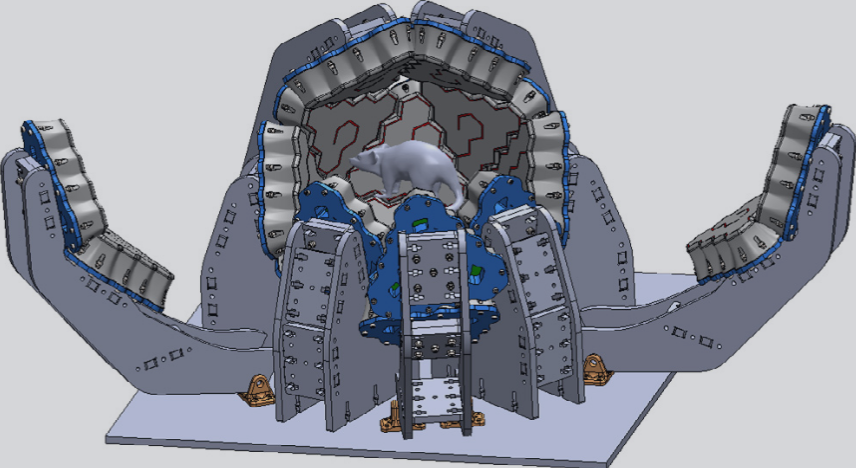
\includegraphics[width=\linewidth]{escaner}
\caption{\textbf{TEMPORAL}Three-dimensional model of the quasi-spherical, hexagonal-based
PET scanner. Reproduced from \cite{perez-benito_sipm-based_2019}.}
\label{fig:escaner}
\end{figure}

The sensitivity of PET is not matched by its spatial resolution. Clinical
scanners typically resolve 4--5\,mm full width at half maximum
(FWHM) \cite{spencer2021}, and
recent advances push the number towards 3\,mm \cite{spencer2021,
gonzalezmontoro2022brain}, higher than the numbers normally achieved with MRI or CT. This limit decomposes into four
contributions, two physical and two belonging to the detector, which behave
very differently from one another \cite{moses2011}. The physical ones are
the finite distance the positron travels before annihilating, set by the
emitting isotope \cite{levin1999}, and the small angular deviation from
antiparallel emission, caused by the residual momentum of the
electron--positron pair. Neither can be engineered away, although the second
translates into a positional error that scales with the diameter of the
detector ring and is therefore smaller in compact systems. The detector terms are more tractable. In pixelated arrays, the size of the
individual element fixes the finest scale at which an interaction can be
localised; shrinking it improves resolution, but the inter-crystal
reflectors then occupy a growing fraction of the detector volume, and the
probability that a photon deposits energy across several elements rises.
The decoding error --- the uncertainty in determining where within the
module the interaction occurred --- amounts to roughly one third of the
detector width \cite{moses2011}. Unlike positron range and non-collinearity,
this term is not a physical floor but a consequence of how the light
distribution is read and interpreted, and it is therefore the one most open to improvement, whether through detector geometry, readout electronics or the algorithms that interpret
the signal.
This is the ground occupied by organ-dedicated scanners. Adapting the
detector geometry to a specific anatomical region increases solid-angle
coverage, and with it sensitivity and resolution, at a lower manufacturing
cost than a general-purpose whole-body system; designs exist for breast,
brain, prostate and cardiac imaging \cite{sanaat2024}. The trade-off is that
irregular geometries complicate calibration and data correction, and that
small gantry apertures accentuate parallax errors and degrade the uniformity
of spatial resolution across the field of view \cite{sanaat2024}. Much of
the design effort in these systems therefore shifts onto the detector
itself.

Our group is currently developing a quasi-spherical brain-dedicated PET
scanner along these lines \cite{perez-benito_sipm-based_2019}. Rather than
the cylindrical ring of conventional systems, its detector modules tile a
closed surface around the head (Fig.~\ref{fig:escaner}), approaching full $4\pi$ steradian coverage
and thereby collecting a far larger fraction of the emitted coincidences
\cite{perez-benito_sipm-based_2019}. The modules are hexagonal, a shape
chosen for two independent reasons: hexagons tile a surface without gaps and
approximate a sphere more closely than square modules of comparable size,
and hexagonal scintillators have also been shown to offer slightly better
light yield and energy resolution than square, triangular or cylindrical
prisms \cite{perez-benito_scintillator_2023}. Each module is built around a monolithic LYSO crystal
\cite{perez-benito_laser-microstructured_2025}.


The choice between segmenting the scintillator and leaving it continuous is
not incidental, and it conditions how the interaction position can be
recovered at all \cite{gonzalezmontoro2022}. In pixelated arrays, the
crystal is cut into individual elements separated by reflectors, so that the
interaction is assigned to whichever element fired. Event positioning is
then simple and fast, but the resolution cannot be finer than the element
itself \cite{moses2011}, and two costs follow from making the elements
smaller: the reflectors occupy a growing fraction of the detector volume,
reducing the packing fraction, and the number of readout channels rises.
Multiplexing schemes, in which several crystals share a readout line and the
position is recovered by decoding the light distribution, are commonly used
to keep this cost manageable \cite{sanaat2024}. Pixelated arrays also
provide no intrinsic depth-of-interaction (DOI) information, which has motivated
layered designs such as phoswich detectors, where stacked scintillators with
different decay times allow a coarse depth assignment at the price of a
degraded timing resolution \cite{sanaat2024}.

Monolithic scintillators take the opposite approach. A single continuous
block is coupled to an array of photodetectors, and the light from each
interaction spreads over many channels at once \cite{gonzalezmontoro2022}. 
Positioning is no longer a matter of identifying an element but of
estimating a coordinate from the recorded light distribution, which shifts
the resolution limit from the geometry of the crystal to the quality of the
positioning algorithm, and makes the DOI recoverable as a
continuous variable \cite{espana_digipet_2014}. The absence of internal reflectors
also restores the packing fraction lost in segmented designs
\cite{sanaat2024}. This is the configuration adopted in the scanner described above, and it is the light sharing across the array that the present work exploits.

\begin{figure}[t]
\centering
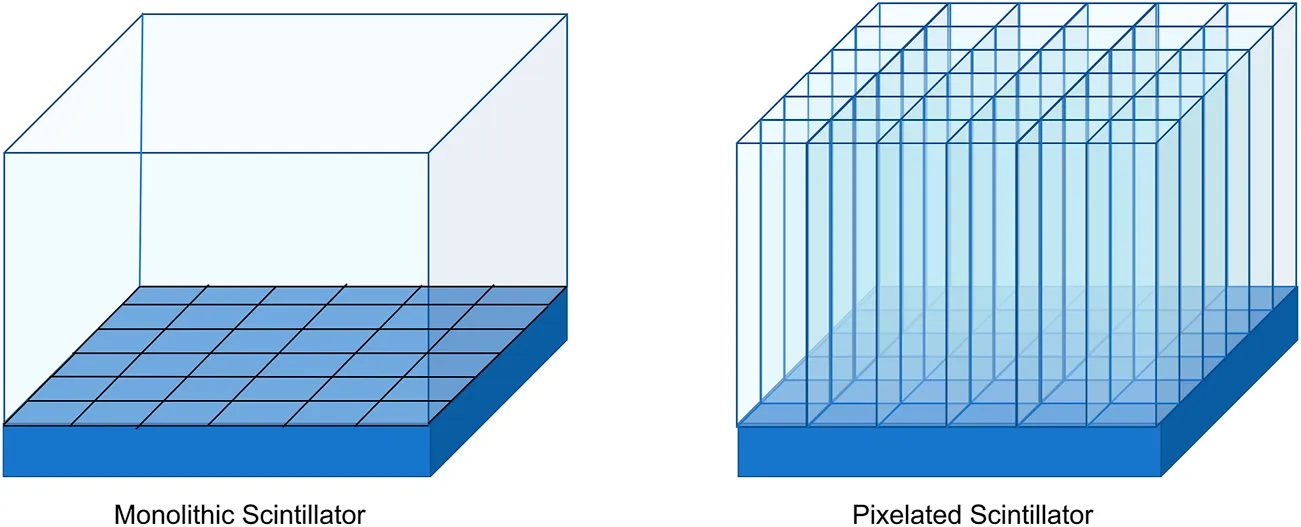
\includegraphics[width=\linewidth]{cristales}
\caption{Monolithic (left) versus pixelated (right) scintillator
configurations. In the monolithic design a continuous slab is coupled to a
segmented photosensor array; in the pixelated design the crystal is cut into
elements coupled one-to-one to the photosensors. Reproduced from
\cite{enlow2023} under CC BY 4.0.}
\label{fig:cristales}
\end{figure}



This light distribution is read out by an array of silicon photomultipliers
(SiPMs) optically coupled to the rear face of the crystal
\cite{gonzalezmontoro2022}. Each interaction produces signal in a subset of
channels, and a readout application-specific integrated circuit (ASIC) amplifies, thresholds and digitises each of them, so that an event is fully described by the vector of charges recorded
across the array. Because a channel only produces an output once it exceeds
the threshold set in the electronics, most entries of that vector are zero
for any given event and only a few channels contribute; the sparsity of the
signal is therefore a property of the acquisition system rather than a
defect of the data \cite{jimenez2025}.

Estimating the interaction position from that vector admits solutions of
widely varying complexity. The most common is the centre of gravity (CoG),
which places the event at the average of the photodetector coordinates,
each weighted by the charge that channel recorded \cite{anger1958}; in
practice the square of the charge is normally used as the weight, which
reinforces the contribution of the channels closest to the interaction point
and improves resolution \cite{poladyan2020}. Its appeal is that it is
deterministic, has no parameters to tune and requires no prior calibration.
In exchange, it exploits only part of the information contained in the light
distribution: recovering the DOI, or correcting the bias
the method itself introduces near the crystal edges, calls for substantially
more elaborate algorithms \cite{conde_minimization_2014}.

The two-dimensional histogram of the positions computed in this way over a
large number of events forms the flood map (Fig.~\ref{fig:floodmap}), in
which the structures engraved in the crystal appear resolved as discrete
spots. It is the image conventionally used to characterise a detector of
this kind, and its sharpness depends on all 61 channels being operational:
the CoG averages over the whole array, and a single missing term is enough
to displace the centroid. The effect is confined to the neighbourhood of the
failing channel --- in the module of Fig.~\ref{fig:floodmap} the
reconstructed position shifts by a median of 0.41\,mm for events within
4\,mm of it, and by less than 0.01\,mm elsewhere --- but within that
neighbourhood the engraved structures are no longer resolved.

\begin{figure}[t]
    \centering
    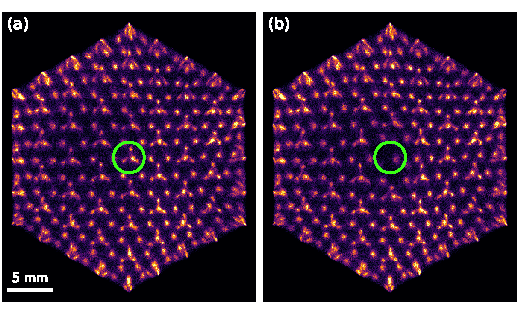
\includegraphics[width=\columnwidth]{floodmap_intro}
    \caption{Flood map of the same detector module reconstructed by centre of
gravity, using the same events in both panels: (a) with all 61 channels
operational and (b) with one channel disabled, marked in green. The
structures engraved in the crystal appear as discrete spots; the inset
magnifies the neighbourhood of the disabled channel.}
    \label{fig:floodmap}
\end{figure}


Silicon photomultipliers degrade and fail for a variety of reasons: thermal
drift, manufacturing defects, deterioration of the optical coupling, or
faults in the readout channel. The consequence for the image is well
recognised in industrial practice: a dead pixel introduces reconstruction
artefacts and incorrect activity values, and commercial systems include
quality-control procedures to identify it \cite{philips2015deadpixel}. The
adopted general solution, however, is to discard the affected information and
compensate for it downstream of positioning, either by duplicating events
from neighbouring pixels in list mode or by interpolating in sinogram space
\cite{philips2015deadpixel}. The channel is not recovered: it is masked out.





This class of problem has motivated the application of deep learning to PET
detector readout \cite{gong2020}. The most developed line is the estimation
of the interaction position in monolithic crystals, where networks trained
on calibration data consistently outperform analytical algorithms and
recover the DOI as a continuous variable
\cite{decuyper2021, jaliparthi2021}. Two previous studies address precisely
this task on the present detector \cite{hidalgo-torres_predicting_2020,
jimenez2025}. All of them share the same framing: the light distribution
recorded by the array is taken as input and the network returns a
coordinate.

Closer to what is proposed here, deep learning has also been applied to
recovering channel signals rather than positions. Networks have been trained
to invert multiplexed readout schemes, reconstructing the individual channel
values from a reduced set of measurements and validating the result on the
recovered flood map \cite{li2023, niu_cnn-based_2024}, and the approach has
recently been extended to semi-monolithic detectors, where the full
64-channel response is reconstructed from 16 row-and-column sums by
exploiting the light sharing between slabs
\cite{loignon-houle_multi-input_2026}. In all these cases, however, the
information carried by each channel is still present in the acquired data:
multiplexing encodes it in a known linear combination, and the network
learns to invert a mapping fixed by design. A failed channel is a different
situation, since nothing of its signal reaches the acquisition and the only
remaining trace of it is the statistical correlation that light sharing
induces among its neighbours.

That situation is not unique to PET. Recovering the response of defective
elements in a sensor array is an established problem in imaging, addressed
either by interpolating from neighbouring pixels or, more recently, by
training autoencoders to reconstruct corrupted regions from their
surroundings \cite{fixpix2023}. The formulation adopted here belongs to that
family: it is the masked autoencoder setting \cite{he2022mae}, in which part
of the input is deliberately hidden and the model is trained to reconstruct
it, which allows supervision to be generated from healthy modules without
requiring labelled faulty detectors. What distinguishes the present case is
that the redundancy being exploited is physical rather than statistical: the
light emitted in a single interaction is measured simultaneously by several
photodetectors, so the value of a channel is constrained by the response of
those around it.

This work proposes to recover that channel rather than discard it. If the
light from each interaction spreads over several photodetectors, the charge
that the failed sensor would have recorded is not entirely lost: it remains
implicit in what its neighbours measured, and the problem is to estimate it.
The difficulty lies less in the model than in the supervision. In a faulty
module there is no way of checking whether an estimate is correct, since the
true charge of the dead channel is unobservable by definition: if it could
be measured, the channel would not be faulty. What cannot be observed,
however, can be simulated. It suffices to take a healthy module, disable one
of its channels and keep the original value as a reference; the fault is
fabricated, and with it the label. The whole approach rests on that idea,
and it is applied to experimental data acquired with the detector described
above rather than to simulations, so that the model learns the behaviour of
the system as it actually is, with its noise, its threshold and its
variation between modules.

The choice of model follows from the geometry of the array. The immediate
option would be to treat the vector of sixty-one charges as a list of
numbers and let a dense network discover on its own which channels are
related to which, but that means learning from scratch something that is
already known: which sensor is adjacent to which. The photodetectors form a
hexagonal tiling in which every interior sensor has six immediate
neighbours, and that neighbourhood is precisely the path along which the
light is shared. A structure of this kind is naturally described as a graph,
with one node per sensor and an edge between each pair of adjacent sensors,
and it therefore admits a neural network that operates on it by propagating
information between neighbours \cite{hamilton2017graphsage}. The model
proposed here follows that approach, incorporating the geometry of the
detector as prior knowledge instead of leaving it implicit in the data.

The evaluation is framed along the same lines. The error in the estimated
charge is the quantity the model minimises, but on its own it says little
about the usefulness of the method: what matters is how much is recovered of
what the fault degrades. Two physical effects are therefore measured: the
displacement of the reconstructed position, which is the direct consequence
on the flood map, and the conservation of the energy spectrum, which
determines whether the restored signal is physically admissible. All of this
on modules the network has not seen during training,
and compared against classical interpolation methods in order to establish
that the complexity of the model is warranted. The behaviour of the method
when more than one channel fails is also examined, with particular attention
to contiguous groups, which are what is observed in real faulty detectors
and the case that displaces the reconstructed position the most, since when an
entire region disappears the lost sensors are left without healthy immediate
neighbours to draw on.

% ---------------------------------------------------------------------
\section{Materials and Methods}
% ---------------------------------------------------------------------

\subsection{Detector and Data}
\label{sec:detector}

Every measurement reported here comes from detector modules of the scanner
described in Section~1. Each module is built around a monolithic LYSO hexagonal
prism, 17.6\,mm on a side and 13\,mm thick, laser-etched into 364 optical
structures that constrain how the scintillation light spreads before reaching
the photosensor \cite{perez-benito_laser-microstructured_2025}. An array of
silicon photomultipliers is optically coupled to its posterior face
\cite{perez-benito_sipm-based_2019}. The array carries 61 photosensors, one per
readout channel, which tile a hexagonal lattice with a pitch of 3.75\,mm and span
26\,mm across, so that the sensors do not reach the crystal boundary. The lateral faces of the crystal carry an absorbing black adhesive
that suppresses edge reflections. This has a consequence that recurs
throughout our results: interactions near the perimeter lose a measurable
fraction of their light, which shifts both the charge recorded by the peripheral
channels and the position of the energy photopeak in those regions.

We used acquisitions recorded with a $^{22}$Na source under flood irradiation,
one file per physical module, comprising 159 healthy modules and 62 modules
with at least one suspected faulty channel. Each file holds on the order of
$10^6$ events. An event activates 17 channels on average, ranging from a single
channel to 54, since a channel only produces an output once it exceeds the
threshold set in the readout electronics. We applied neither energy calibration
nor an energy window. Both would require a per-channel calibration that is not
available for this set of modules, and the metric we use to assess spectral
fidelity is constructed so that their absence cancels, as
Section~2.6 explains.

We split the healthy modules by file rather than by event, with a fixed seed:
149 for training, 5 for validation and 5 held out for testing. The distinction
matters more than it might appear. Each file is a different physical detector,
with its own gain, its own optical coupling and its own defects, so splitting
by file measures generalisation to hardware the model has never seen. Splitting
by event would let the model learn the idiosyncrasies of a detector and then be
tested on that same detector, which is a considerably easier problem and not
the one that arises in practice. The test partition was reserved before any
training and used neither for fitting nor for model selection.

\subsection{Preprocessing and Sample Generation}
\label{sec:preproc}

The raw quantity is a vector $\mathbf{r} \in \mathbb{R}^{61}$ holding the
digitised charge of each channel for one event. We applied two operations
before it reaches the network. Occasional negative values, produced by baseline
subtraction in the electronics, were clipped to zero, since a negative charge
has no physical meaning and would distort the centroid. Events in which no
channel exceeded the threshold carry no information and were discarded.

We then simulated a faulty channel by forcing a subset $\mathcal{D}$ of the
entries to zero and asking the model to recover the original vector from what
remained. The network additionally receives a binary mask indicating which
entries were suppressed, so that a channel switched off is distinguishable from
a channel that legitimately recorded no signal. This is the masked autoencoder
setting \cite{he2022mae} applied to detector channels instead of image patches,
and it makes the supervision self-generated: the target is the original vector,
so no module with a genuinely dead sensor is needed for training. We drew a
fresh $\mathcal{D}$ for every sample, so a given event is never seen twice with
the same failure pattern.

Normalisation, however, deserves a comment, because it constrains the
architecture. We scaled each event by the maximum of its own masked vector,
%
\begin{equation}
\mathbf{x} = \frac{\tilde{\mathbf{r}}}{\max_{c} \tilde{r}_{c}},
\qquad
\mathbf{y} = \frac{\mathbf{r}}{\max_{c} \tilde{r}_{c}},
\label{eq:norm}
\end{equation}
%
where $\tilde{\mathbf{r}}$ is the masked vector and $\mathbf{y}$ the target.
Two choices are embedded here. Scaling per event rather than per dataset
follows from the physics: for position estimation what matters is how the light
distributes across the array, not how much light the interaction released.
Computing the factor \emph{after} masking means that the target of a suppressed
channel exceeds unity whenever that channel was the brightest of the event.
The output layer is therefore linear, with no sigmoid or clamp, because
bounding it would make the brightest failures unrecoverable by construction.

One further choice concerns which channel to suppress. Roughly three quarters
of the channels in any given event are below threshold, so drawing the seed
uniformly would produce a training set in which most samples require no
correction at all, and the model would reasonably learn to predict zero. We
therefore balanced the draw: half of the samples suppress a channel that
carried signal and half suppress a channel already at zero.

\subsection{Failure Regimes}
\label{sec:regimes}

A single dead channel is the simplest fault, but not the only one. When we
inspected the flood maps of the 62 defective modules, we found three recurring
patterns. What matters is not so much how many sensors fail as how they are
arranged: one whose neighbours are all healthy can be reconstructed from them,
whereas one surrounded by other dead sensors cannot.

We reproduced those patterns with three mask-generation strategies, illustrated
in Fig.~\ref{fig:regimenes-diagrama}. In the \emph{cluster} regime the $k$
suppressed channels grow outward from the seed so that they remain contiguous,
so an entire region of the array disappears at once and the affected sensors
are left without healthy immediate neighbours. In the \emph{scatter} regime
they are drawn uniformly across the array, so each failure is effectively
isolated. The \emph{near} regime sits between the two: the $k$ channels lie
within two hops of the seed without being required to touch. That intermediate case is the one we observed most often in real faulty
modules, typically two or three sensors separated by one or two positions, and
it is the reason we introduced it rather than settling for the two extremes.

\begin{figure}[t]
\centering
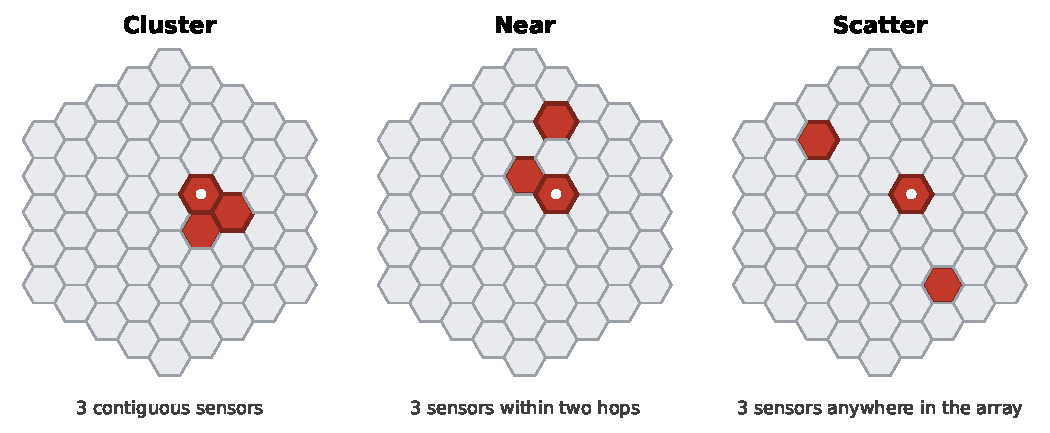
\includegraphics[width=\linewidth]{regimenes_diagrama}
\caption{The three failure regimes used to generate the training masks, shown
on the 61-sensor array for $k=3$. Suppressed sensors are marked in red and the
white dot indicates the seed from which the pattern grows. Cluster forces the
failures to be contiguous, scatter distributes them across the array, and near
places them within two hops of the seed without requiring contact.}
\label{fig:regimenes-diagrama}
\end{figure}

\subsection{Network Architecture}
\label{sec:arch}

The geometry of the array suggests how to model the problem. A dense network
receiving the 61 charges as a flat vector would have to learn which sensors are
adjacent, something already known from the physical layout. We therefore
represented the detector as a graph whose nodes are the 61 active sensors and
whose edges join physically adjacent ones, and propagated information along
those edges \cite{gilmer2017mpnn, hamilton2017graphsage}. The resulting
adjacency has 312 directed edges, with 37 nodes of degree six, 18 of degree
four and 6 of degree three, and it is fully symmetric.

Each layer of our model, which we refer to as HexGNN, updates a node from its
own state and the mean of its neighbours,
%
\begin{equation}
h_{c}^{(l+1)} = \sigma\!\left( W_{s} h_{c}^{(l)}
  + W_{n} \frac{1}{|\mathcal{N}(c)|} \sum_{j \in \mathcal{N}(c)} h_{j}^{(l)}
  + b \right),
\label{eq:hexconv}
\end{equation}
%
where $\mathcal{N}(c)$ are the neighbours of sensor $c$ and $\sigma$ is a Gaussian error
linear unit (GELU) \cite{hendrycks2016gelu}. The aggregation is isotropic: every
neighbour of a node shares the weight matrix $W_{n}$, so the layer encodes
adjacency but not direction. Batch normalisation \cite{ioffe2015batchnorm} is
applied between blocks. Our reference configuration uses a hidden width of 48
and four blocks, for \num{38305} trainable parameters.

We compared this model against three groups of alternatives. As classical
baselines without learned parameters we used the mean of the neighbouring
channels and a per-channel linear regression on the remaining 60, both fitted
on training modules only and both excluding the target channel from their
inputs. As neural baselines without a geometric prior we trained a deep multilayer
perceptron and a residual multilayer perceptron with channel attention. Both
receive the same information but no notion of adjacency, which isolates the
contribution of the prior from that of raw capacity.


The aggregation in Eq.~\ref{eq:hexconv} is deliberately simple, and it is fair
to ask whether that simplicity is what limits performance. We therefore tested
four alternatives, each addressing a different suspicion about where the
bottleneck might be.

If the six neighbours of a sensor contribute unequally --- and they might, since
the light reaching one of them depends on the direction of the interaction ---
then averaging them discards useful information. Graph attention networks (GAT)
\cite{velickovic2018gat} learn a weight per neighbour instead of fixing it,
which lets the model decide how much each one should count. A related but
broader concern is that the mean is only one summary of a neighbourhood.
Principal neighbourhood aggregation (PNA) combines several statistics and
scales them by node degree, retaining information that any single one throws
away \cite{corso2020pna}; degree varies here between three and six, so the
scaling is not vacuous.

The other two alternatives question the locality of the model rather than its
aggregation. Our layers propagate information one hop at a time, so with four
blocks a sensor only sees four rings away. If the missing charge were
constrained by the global shape of the light distribution, a wider receptive
field would help. We tested this in two forms: a graph U-Net, which pools the
graph into a coarser representation before expanding it back
\cite{gao2019graphunet}, and a graph transformer (Graphormer) in which every
node attends to every other one regardless of adjacency
\cite{ying2021graphormer}. We also tested metric edge features, anisotropic
hexagonal convolution with one weight per direction, per-channel equalisation,
heteroscedastic prediction of mean and variance, and averaging ensembles
\cite{lakshminarayanan2017ensembles}.

\subsection{Training}
\label{sec:training}

We trained with the mean squared error (MSE) computed over the full 61-channel
output rather than the suppressed entries alone,
%
\begin{equation}
\mathrm{Loss}_{\mathrm{MSE}} = \frac{1}{61} \sum_{c=1}^{61}
              \left( \hat{y}_{c} - y_{c} \right)^{2},
\label{eq:loss}
\end{equation}
%
which treats the task as ordinary regression and keeps the healthy channels as
a consistency constraint.

We chose it after comparing it against the mean absolute error (MAE) and the
Huber loss \cite{huber1964}, which interpolates between the two by behaving
quadratically for small residuals and linearly for large ones,
%
\begin{equation}
\mathrm{Loss}_{\delta}(e) =
\begin{cases}
\tfrac{1}{2} e^{2} & \text{if } \lvert e \rvert \le \delta, \\[2pt]
\delta \left( \lvert e \rvert - \tfrac{1}{2}\delta \right) & \text{otherwise,}
\end{cases}
\label{eq:huber}
\end{equation}
%
with $e = \hat{y}_{c} - y_{c}$ and $\delta = 0.1$. The motivation for testing it
is that the targets contain legitimate extreme values, since a suppressed
channel that was the brightest of its event has a target above unity, and a
quadratic penalty weights those cases heavily. In practice the MSE gave the
lower bias, which is the property we were unwilling to trade, so it is the loss
used throughout.

We also tested two physics-informed variants, one penalising the displacement
of the reconstructed position and one penalising the shift of the energy
spectrum; both are reported in Section~\ref{sec:res-negative}.

Table~\ref{tab:hyperparams} lists the configuration. Two aspects of the
procedure are worth making explicit. First, the training set does not fit in
memory, so modules are loaded one at a time and contribute \num{107000} events
each; the model therefore performs a single pass over \num{15943000} masked
samples. Since the masks are regenerated for every sample, no exact input is
ever repeated, which is why we applied no early stopping. Second, we selected
the final weights by the validation error on the imputed channel, computed on
a fixed set of \num{400000} events with a fixed mask seed. We did not use the
total loss for this purpose. It is dominated by the 60 healthy channels and
stays nearly flat across the run, so it separates checkpoints poorly.

\begin{table}[t]
\centering
\caption{Training configuration of the reference model.}
\label{tab:hyperparams}
\begin{tabular}{@{}ll@{}}
\toprule
\textbf{Parameter} & \textbf{Value} \\
\midrule
Architecture        & HexGNN, 4 blocks, hidden width 48 \\
Trainable parameters & \num{38305} \\
Activation          & GELU \\
Loss                & MSE over the 61 channels \\
Optimiser           & AdamW \cite{loshchilov2019adamw} \\
Learning rate       & $10^{-3}$, cosine decay \cite{loshchilov2017sgdr} \\
Weight decay        & $10^{-4}$ \\
Batch size          & 512 \\
Training samples    & \num{15943000} (single pass) \\
Validation events   & \num{400000}, fixed masks \\
Model selection     & Validation MAE on the imputed channel \\
\bottomrule
\end{tabular}
\end{table}

Each run stores its preprocessing configuration inside the checkpoint. This is
a safeguard rather than a detail: a model trained with one normalisation and
evaluated with another produces meaningless numbers without raising any error,
and verifying the match automatically removes that failure mode.

\subsection{Evaluation Metrics}
\label{sec:metrics}

The quantity the model minimises is the error in the recovered charge, but on
its own it says little about whether the method is useful. What matters is how
much of the degradation caused by the fault is undone. We therefore evaluated
on three levels: the charge itself, the position it produces, and the physical
quantities the detector is built to deliver.

At the charge level we report, over the $N$ events in which channel $c$ was
suppressed, the MAE and the bias
%
\begin{equation}
\mathrm{MAE}_{c} = \frac{1}{N} \sum_{i=1}^{N} \lvert \hat{y}_{i} - y_{i} \rvert,
\qquad
\mathrm{bias}_{c} = \frac{1}{N} \sum_{i=1}^{N} (\hat{y}_{i} - y_{i}),
\label{eq:mae}
\end{equation}
%
both in the normalised units of Eq.~\ref{eq:norm}. The bias acts as a
guardrail. A model can attain a low MAE while predicting systematically low,
which would displace every reconstructed position in the same direction; only
the signed average reveals it. Because a normalised error is hard to interpret
on its own, we also express the MAE relative to the mean charge that the
channel collects. That ratio is sensitive to the number of events used for the
denominator, so we computed numerator and denominator on the same sample
throughout.

The position level is our primary metric, since it is the one that reaches the
image. For each event we computed the interaction position by CoG weighted by
the squared charge \cite{anger1958, poladyan2020}, in three versions of the
same event: intact, with the channel suppressed, and with the channel imputed.
Comparing them against the intact position gives two displacements. The
\emph{degraded} displacement $\Delta R_{\mathrm{deg}}$ is how far the centroid
moves when the fault goes uncorrected, and therefore measures the damage. The
\emph{imputed} displacement $\Delta R_{\mathrm{imp}}$ is how far it still lies
from the true position after the model has acted, and therefore measures the
residual error. Recovery is the fraction of the damage the model removes,
%
\begin{equation}
\mathrm{Recovery} = 100 \times
  \left( 1 - \frac{\Delta R_{\mathrm{imp}}}{\Delta R_{\mathrm{deg}}} \right),
\label{eq:recovery}
\end{equation}

%Declara percentil 90 como siglas y cambialo en todo por P90, más legible. [Checked]
with both terms evaluated at the same quantile and over the same population of
events. A value of 100\,\% would mean the imputed position coincides with the
intact one, and 0\,\% that imputing changed nothing. We report the value at the
90th percentile (P90), which weights the difficult events, and also the mean.
Averaging over the 61 channels gives the macro figures used throughout, and the
minimum over channels characterises the worst case. Since a ratio says nothing
about the magnitude of what remains, we also report
$\Delta R_{\mathrm{imp}}$ in millimetres.

Two further analyses ask a different question. Recovery tells us how close the
imputed position is to the true one, but not whether the restored signal is
physically admissible. A model could place events correctly on average while
distorting the quantities the detector is built to measure.

The first analysis characterises the \emph{spread} of the positioning error
rather than its typical size. Recovery reports a percentile of $\Delta R$; here
we summarise the same underlying distribution by its width, taking the error
components $\Delta x$ and $\Delta y$ and computing a Gaussian-equivalent full
width at half maximum from a robust scale estimate,
%
\begin{equation}
\mathrm{FWHM} = 2.3548 \cdot \tfrac{1}{2}
  \left( \hat{\sigma}_{\Delta x} + \hat{\sigma}_{\Delta y} \right),
\qquad
\hat{\sigma}_{v} = 1.4826 \cdot \mathrm{MAD}(v),
\label{eq:fwhm}
\end{equation}
%
where MAD denotes the median absolute deviation, used so that a few extreme
events do not drive the estimate. Alongside it we report the bias
$\lVert(\overline{\Delta x}, \overline{\Delta y})\rVert$, which separates a
systematic displacement of the map from a symmetric blurring around the correct
position.

%Esto no lo veo del todo pero bueno, osea entiendo el point pero explica mejor el punto de porque usamos el FWMH. [Checked]
Reporting the width alongside the percentile serves a specific purpose: it
splits the error into two components that behave differently. The bias is a
systematic shift of the whole distribution and is in principle correctable,
because it is predictable from the surviving channels. The width is random
scatter around that shift, and no amount of information from the neighbours
removes it. A model can be good at one and poor at the other, so we report them
separately.

One clarification is needed because the name invites it. This FWHM is not the
spatial resolution of the detector: it is computed on the error that the fault
introduces, not on the point-spread function of the system, and the two differ
by about two orders of magnitude. It is also not independent of
Eq.~\ref{eq:recovery}, since both summarise the same distribution of
positioning errors.

The second concerns energy. Suppressing a channel removes part of the collected
light, so the reconstructed energy of the event falls and the photopeak shifts
towards lower values; a good imputation should put it back. Measuring this is
complicated by the absence of energy calibration, since we cannot convert
ADC counts into keV. We avoided the problem with a paired differential design:
over the same events we subtract the true charge of the channel and add back
the prediction, so any calibration factor multiplies both terms and cancels.
We evaluated this by zones of the crystal, defined as concentric hexagonal
bands, because the absorbing adhesive on the lateral faces makes the periphery
behave differently from the centre \cite{conde_minimization_2014} and an
average over the whole crystal would hide that difference.

%Exceso de honestidad, Lidia hace algo asi? no hace falta decirlo todo no?. [Checked]
Every model is evaluated on the same modules, the same events and the same
masks, so that differences between models are measured on paired samples.
Section~\ref{sec:res-variability} quantifies how far that precision extends.

%Acabo de ver que Lidia habla de implementation details, convendría poner una pequeña seccion similar, todo se ha hecho con python con datos reales de [Checked]
%en Python, con Pytorch, Matplotlib, etc.. además se ha usado una 1660 super y Ryzen 5 3600x. [Checked]
\subsection{Implementation Details}
\label{sec:implementation}

We implemented the models in PyTorch, and the data pipeline, the evaluation and
the figures in Python with NumPy, SciPy and Matplotlib. Training ran on a single
NVIDIA GeForce GTX 1660 SUPER with an AMD Ryzen 5 3600X personal computer.


% ---------------------------------------------------------------------
\section{Results}
\label{sec:results}
% ---------------------------------------------------------------------

%Este parrafo lo veo un poco inutil no se se puede reducir, e introducir en el parrafo siguiente. [Checked]
%Lo de las evaluation campagnes ni lo menciones no creo que sea necesario. [Checked]
\subsection{Imputation Accuracy}
\label{sec:res-accuracy}

%esta muy bien pero si es para un solo canal esta seccion dejarlo claro con un single y n=4 entiendo que de modelos, para dejarlo claro. [Checked]
This section reports a single suppressed channel, which is the failure mode the
method targets; the multi-channel case follows in
Section~\ref{sec:res-multidead}. Every value is the mean over four
independently trained models evaluated on the five held-out modules, and the
stated deviation is the spread between those models.

%Respeta las siglas una vez invocadas. [Checked] auditadas las 15 siglas del documento: 0 formas largas repetidas
The reference model recovers the charge of a suppressed channel with a MAE of $0.6228 \pm 0.0064$ in normalised units. Expressed relative to
the mean charge that each channel collects, this amounts to a 29.1\,\% error,
and it is not uniform across the array: 25.9\,\% for channels in the core of the
crystal against 34.0\,\% at the edge. The absorbing adhesive on the lateral
faces accounts for that gap, since peripheral channels collect less light and
their neighbours carry correspondingly less information about them.

%Perfecto he cambiado una cosilla para hacerlo más natural. 
The bias stays at $-0.062 \pm 0.023$, that is, below a tenth of the MAE. This
matters because the failure mode we were guarding against is a model that
minimises its error by predicting conservatively low values, which would look
acceptable in the MAE and would systematically displace the reconstructed
position but does not happen in the experiments. 
%Nota para mi: Basicamente si el Bias=MAE el modelo sería conservador y tendría una tendencia a corregir erronea
\subsection{Recovery of the Reconstructed Position}
\label{sec:res-position}

%v2.1: He cambiado un par de cosas que me sonaban raro. 
Charge error is an good indicator, but what reaches the image is the
displacement of the centroid, and Table~\ref{tab:position} gives it in
millimetres. Suppressing a channel moves the reconstructed position of the
affected events by a median of 0.099\,mm and, for the worst tenth of them, by
0.666\,mm. After imputation those figures fall to 0.047\,mm and 0.283\,mm, so
the residual displacement at P90 is 7.5\,\% of the 3.75\,mm sensor pitch. The
degraded column is identical across the four models, since it
does not depend on the imputation; it serves as a consistency check on the
evaluation.

\begin{table}[t]
\centering
\caption{Displacement of the reconstructed position with respect to the intact
event, before and after imputation. Mean $\pm$ standard deviation over four
independently trained models. The degraded column does not depend on the model
and is therefore identical in the four.}
\label{tab:position}
\begin{tabular}{@{}lccc@{}}
\toprule
 & \textbf{Degraded (mm)} & \textbf{Imputed (mm)} & \textbf{Recovery (\%)} \\
\midrule
Median & 0.099 & $0.047 \pm 0.001$ & $50.22 \pm 1.82$ \\
Mean   & 0.241 & $0.117 \pm 0.001$ & $52.15 \pm 0.31$ \\
P90    & 0.666 & $0.283 \pm 0.004$ & $58.04 \pm 0.37$ \\
\bottomrule
\end{tabular}
\end{table}

Fig.~\ref{fig:linediff} shows what this means for the image. Each panel is the
difference between a flood map and the intact reference, averaged over failures
of the sensors along one line of the array. Without correction the difference
covers the neighbourhood of the failing channel with a pattern of excess and
deficit counts, which is the signature of events being displaced towards the
surviving sensors, as the CoG express. After imputation that pattern largely disappears. The lower
row, which follows a line towards the edge of the crystal, shows a residual
that the upper row does not: the periphery is where the method has least
information to work with, as explained in the per-channel errors of
Section~\ref{sec:res-accuracy}.

\begin{figure*}[t]
\centering
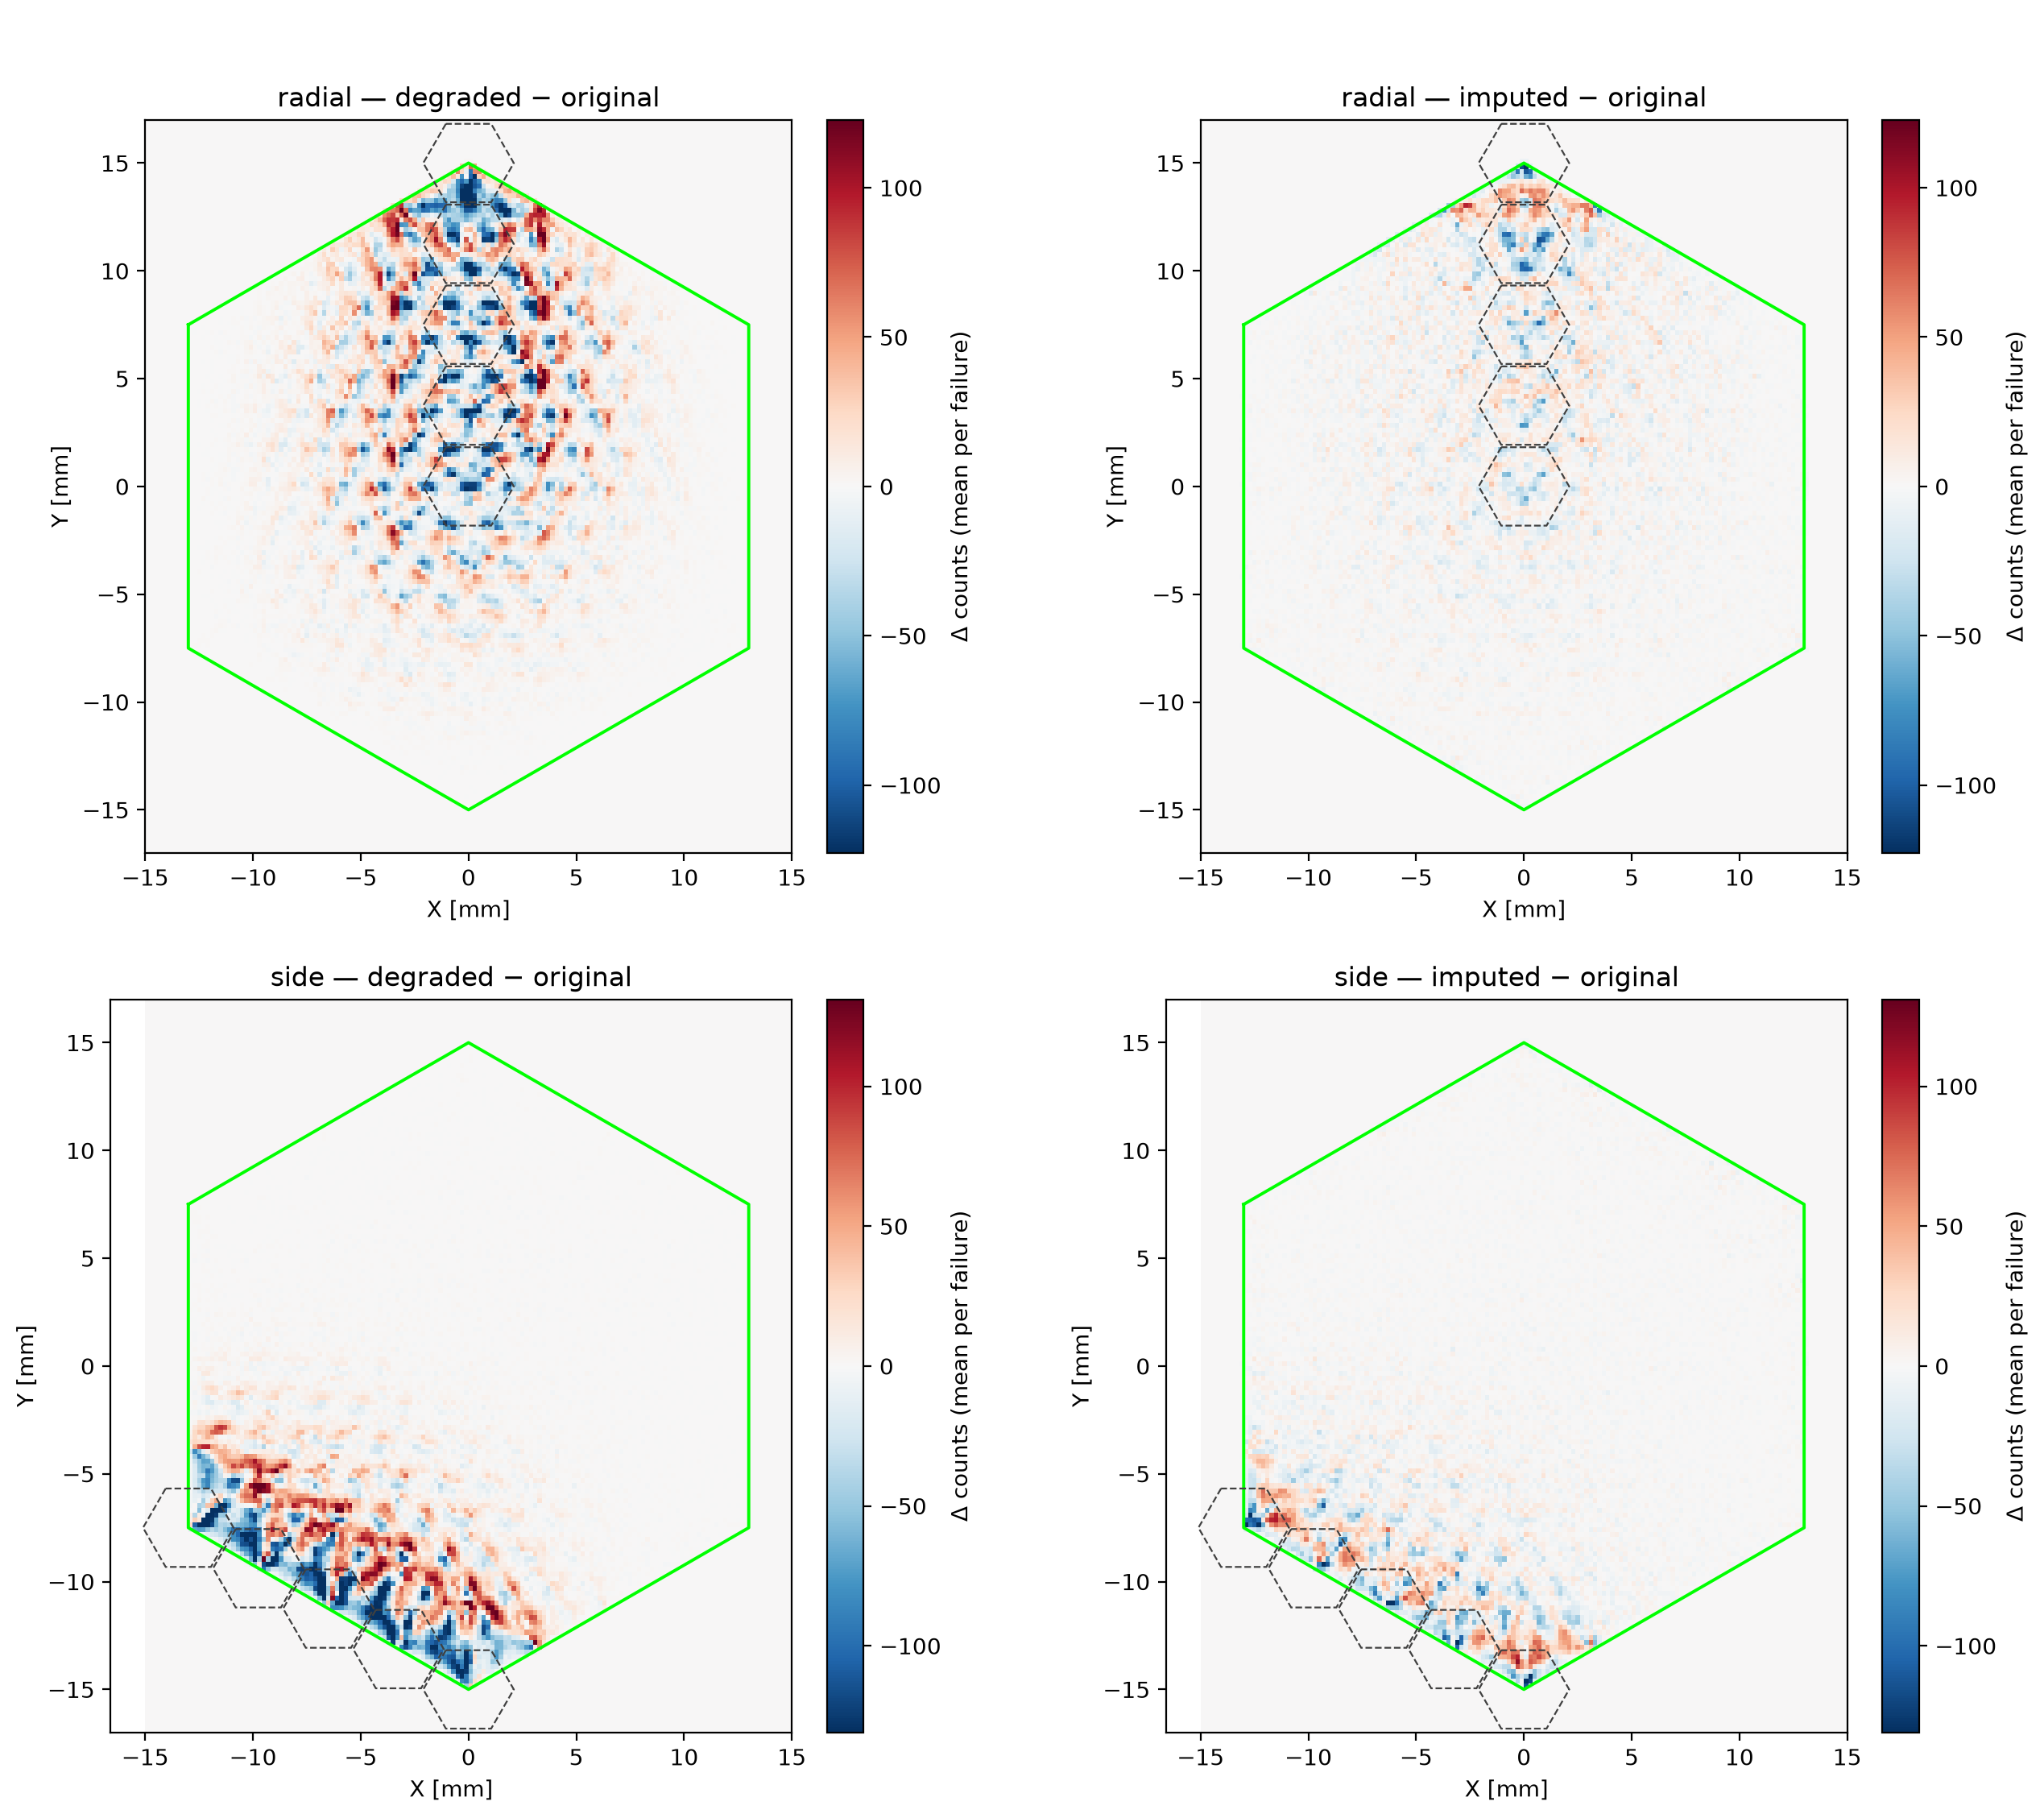
\includegraphics[width=0.92\textwidth]{line_floodmap_diff}
\caption{Average flood-map distortion caused by the failure of a sensor.
Each panel shows the difference in counts with respect to the intact map: red
where the fault adds events and blue where it removes them. Top row, sensors
along a radial line; bottom row, sensors along a line towards the edge. Left,
without correction; right, after imputation. The dashed hexagons mark the
sensors involved and the green outline the crystal boundary.}
\label{fig:linediff}
\end{figure*}


Performance is not uniform across the detector. Fig.~\ref{fig:mapa} maps the
recovery of each of the 61 channels and reproduces the same core-to-edge
gradient. Central channels, whose light is shared with six neighbours, exceed
60\,\%; channels on the perimeter, with three or four neighbours and less
collected light, fall below 45\,\%.

\begin{figure*}[t]
\centering
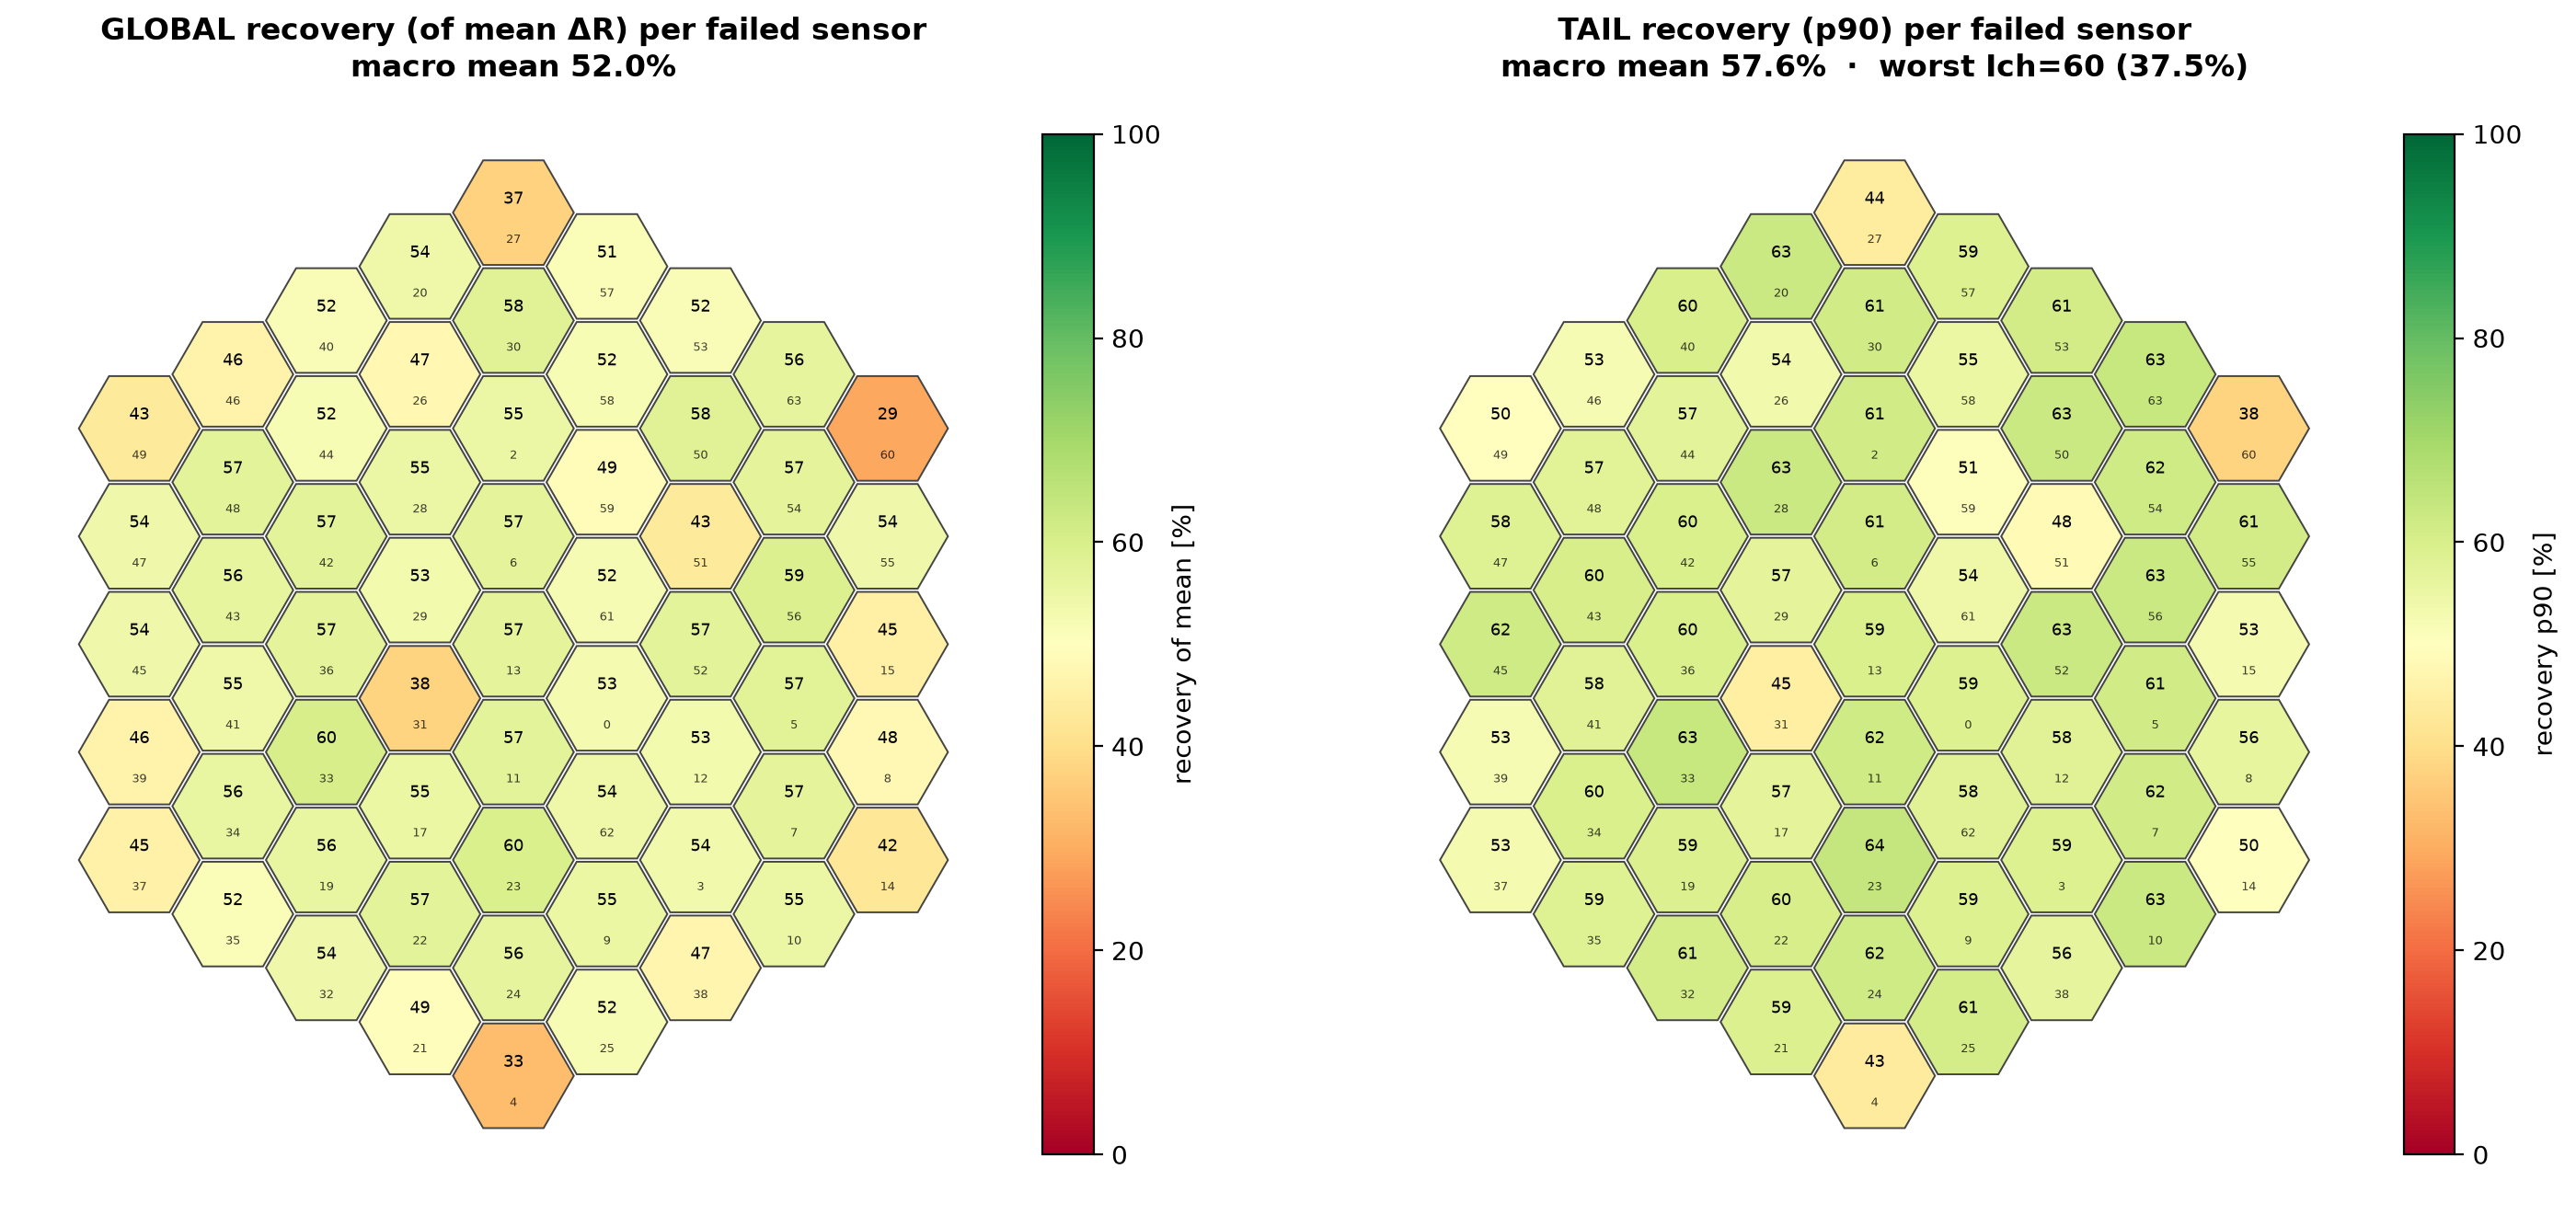
\includegraphics[width=0.92\textwidth]{mapa_recuperacion}
\caption{Recovery per channel over the 61 active sensors, at the 90th
percentile (left) and on average (right). The colour scale is common to both
panels. Recovery degrades towards the perimeter of the array.}
\label{fig:mapa}
\end{figure*}

Fig.~\ref{fig:floodmap-res} closes the sequence with the flood map itself,
where the practical consequence is visible: the etched structures around the
failing channel, which the fault blurs into one another, are resolved again
after imputation.

\begin{figure*}[t]
\centering
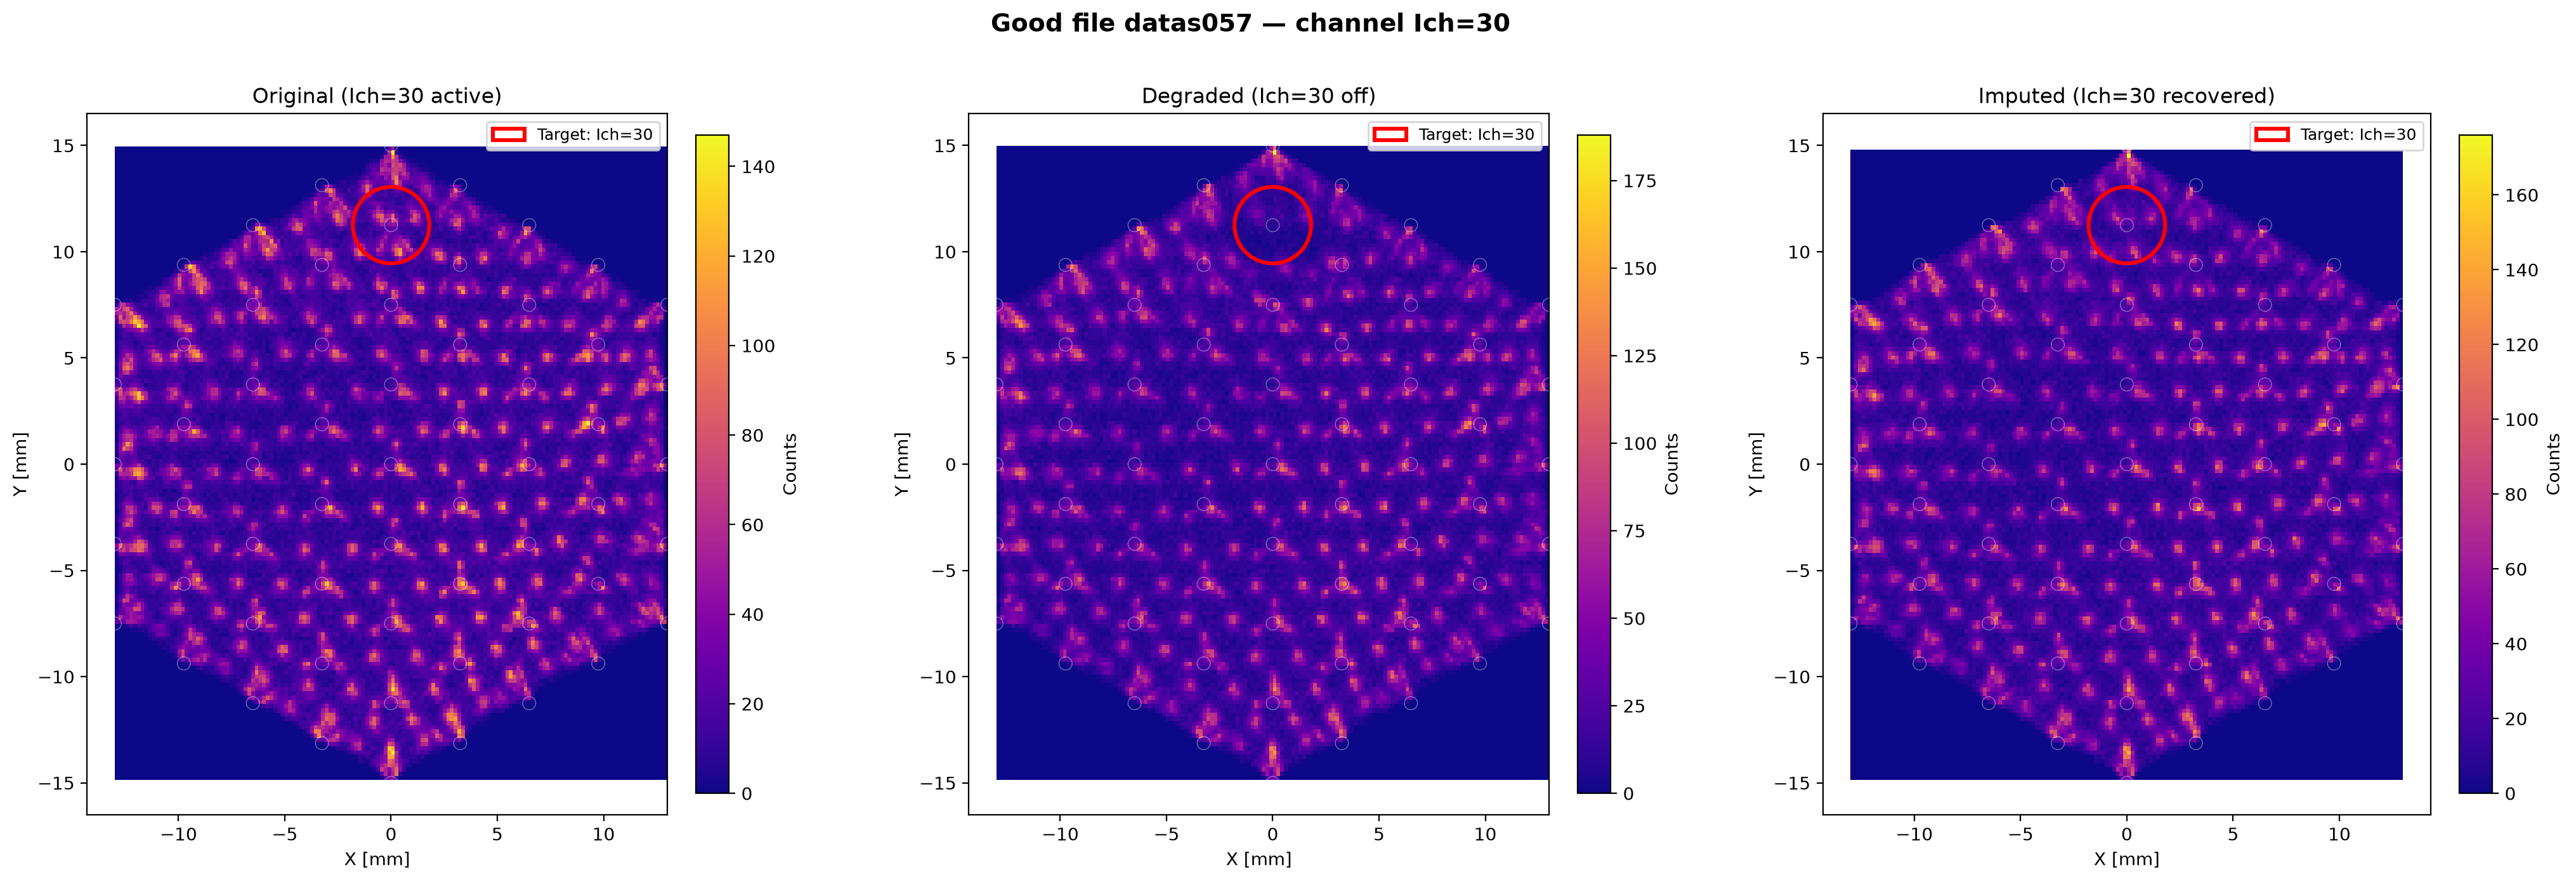
\includegraphics[width=0.92\textwidth]{floodmap.png}
\caption{Flood map of a test module reconstructed from the same events. Left,
with all 61 channels operational; centre, with one channel disabled; right,
after imputing it.}
\label{fig:floodmap-res}
\end{figure*}

\subsection{Value of the Geometric Prior}
\label{sec:res-prior}

Table~\ref{tab:architectures} compares the architectures under a common
evaluation. The two models without a geometric prior reach 51.39\,\% and
48.92\,\% recovery at P90. The smallest graph model reaches
58.0\,\% with an order of magnitude fewer parameters than either of them.

\begin{table}[t]
\centering
\caption{Architecture comparison under a common evaluation campaign. Recovery
at P90 and on average, in per cent; MAE in normalised units.}
\label{tab:architectures}
\begin{tabular}{@{}lrccc@{}}
\toprule
\textbf{Model} & \textbf{Params} & \textbf{Rec.\ p90} & \textbf{Rec.\ mean} & \textbf{MAE} \\
\midrule
DeepMLP           & \num{500541}  & 51.39 & 45.90 & 0.7219 \\
ResidualMLP       & \num{345981}  & 48.92 & 44.81 & 0.7299 \\
Graphormer        & \num{4263881} & 55.17 & 49.65 & 0.6600 \\
Graph U-Net       & \num{331649}  & 55.22 & 47.95 & 0.6918 \\
PNA               & \num{165761}  & 58.45 & 52.48 & 0.6309 \\
\textsc{HexGNN-s} & \num{38305}   & 58.02 & 52.66 & 0.6195 \\
\textsc{HexGNN-m} & \num{225217}  & 58.27 & 52.64 & 0.6185 \\
\textsc{HexGNN-l} & \num{398593}  & 57.47 & 51.96 & 0.6385 \\
\bottomrule
\end{tabular}
\end{table}
%Creo que aqui se podría mencionar que metodo es cual, decir los nombres. [Checked]
Neither capacity nor a more elaborate aggregation moves that figure. Widening
\textsc{HexGNN} from 38\,k to 399\,k parameters changes recovery by less than a
point in either direction. The two architectures with a wider receptive field
perform three points \emph{worse}: Graphormer reaches 55.17\,\% with 4.3\,M
parameters and the graph U-Net 55.22\,\% with 332\,k, against 58.02\,\% for the
38\,k reference. PNA, which combines several aggregation statistics scaled by
node degree, matches the reference at 58.45\,\% rather than exceeding it, using
four times as many parameters. The problem behaves as a local
one, and the isotropic mean over immediate neighbours is enough to solve it.

To test whether the advantage comes from the detector geometry rather than from
message passing in general, we retrained the reference with the adjacency
randomly permuted, preserving the number of nodes, the number of edges and the
degree distribution. The graph is then equally connected but physically
meaningless. Recovery collapses to 28.08\,\%, 27.66\,\% and 31.28\,\% across three
independent permutations, roughly half of the 58.0\,\% obtained with the true
adjacency. The prior therefore accounts for about thirty points of the sixty
the model achieves, and it is the specific adjacency of the detector that
matters, not the fact of using a graph.

Against methods without learned parameters the network recovers 57.9\,\%,
compared with 45.41\,\% for the method that applies the mean of the neighbouring channels and
46.56\,\% for a per-channel linear regression on the remaining 60. The margin
is 12.49 and 11.33 percentage points respectively, which answers the question
of whether the complexity of the model is warranted.

The linear baselines also let us measure how far the useful information
extends. Restricting the regression to the first ring of neighbours, 5.1
channels on average, gives 44.04\,\% recovery. Adding the second ring, 13.7
channels, raises it to 46.42\,\%. The third ring adds 0.09 points and using all
60 remaining channels adds a further 0.04. Beyond the second ring there is
essentially nothing left to extract, which is consistent with a model whose
layers propagate information only a few hops.

\subsection{Generalisation and Variability}
\label{sec:res-variability}
%Esta intro poetica?? Mejor algo como, para hacer un analisis estadistico riguroso de los modelos.... [Checked]
To characterise the uncertainty of the reported figures we measured the two
sources of variability separately (Table~\ref{tab:reference}). Both refer to
the reference configuration used throughout this section: \textsc{HexGNN-s}
trained with the MSE on single-channel failures, evaluated on the five held-out
modules. Across four independent training runs on a fixed partition, differing
in the global seed and in the order in which the modules are presented,
recovery at P90 is $58.04 \pm 0.37$\,\%.

\begin{table}[t]
\centering
\caption{Sources of variability in the reference model. Values are
mean $\pm$ standard deviation over $n$ independent runs.}
\label{tab:reference}
\begin{tabular}{@{}lccc@{}}
\toprule
\textbf{Source of variation} & \textbf{$n$} & \textbf{Rec.\ p90} & \textbf{Rec.\ mean} \\
\midrule
Training run, fixed partition & 4 & $58.04 \pm 0.37$ & $52.15 \pm 0.31$ \\
Data partition                & 5 & $56.56 \pm 2.32$ & $50.60 \pm 2.04$ \\
\bottomrule
\end{tabular}
\end{table}
% De nuevo creo que no queda claro el modelo de referencia que se esta usando. [Checked]
Repeating the experiment with five different partitions of the same 159
modules, however, gives $56.56 \pm 2.32$\,\%, a standard deviation six times
larger. Evaluating the model on individual unseen modules explains why:
recovery ranges from
29.2\,\% to 63.0\,\% depending on which detector it is measured on, with a
standard deviation of 7.86 percentage points across modules. With five modules
in the test partition, that places the standard error of the reported mean at
3.5 points.

%Esta frase no me gusta tampoco, Is worth to be developed/explained/discussed... [Checked]
%%%La frase final esta bien pero todo lo anterior esta un poco lioso. [Checked]
Which of the two bands applies depends on the question. When two models are
compared, the comparison is paired --- the same modules, the same events and the
same masks --- so the band that applies is the $\pm 0.37$ of the training run,
and differences of tenths of a point are real. When the question is instead how
the method will behave on a detector nobody has measured, the band that applies
is the $\pm 2.32$ of the partition, because what dominates there is which
detectors happen to fall in the test set and not anything about the training.
We therefore take $56.56 \pm 2.32$\,\% as the figure that describes
what the method achieves on unseen hardware.

%Que significa to use as a claim, osea demuestralo pero tampoco juzgues aqui, que el [Checked]
%que lo lea diga si esa varianza es legal o demasiado. 
The minimum over the 61 channels behaves in the same way, only more so. Over
four independent runs it averages $42.29 \pm 4.45$\,\%, spanning 37.54\,\% to
47.76\,\%, and the channel that attains it is not the same in every run:
$\mathrm{Ich}\ 60$ in two of them and $\mathrm{Ich}\ 31$ in the other two. Its
deviation across runs is twelve times that of the macro average computed over
the same four runs.

\subsection{Multiple Simultaneous Failures}
\label{sec:res-multidead}
%v2.1 Esta seccion en general esta un poco mal explicada, es dificil seguirla mira los comentarios que te dejo. [Checked]
% Reescrita entera. El problema de fondo era que "cluster", "near" y "scatter"
% designan dos cosas a la vez -con que geometria se ENTRENA y con cual se
% EVALUA- y el texto saltaba de una a otra sin avisar. Ahora la tabla lo
% etiqueta explicitamente y el texto no usa nunca "intermediate regime".

Two questions arise once more than one channel fails at a time: whether a model
trained on single failures still works, and whether the geometry used to
generate the training masks matters. They are separate questions, and
Table~\ref{tab:multidead} answers both. Its rows are the geometry a model was
\emph{trained} on and its columns the geometry it is \emph{evaluated} on, so the
diagonal is each model on its own terrain.

\begin{table}[t]
\centering
\caption{Recovery at P90 averaged over $k=1\dots4$ suppressed channels, over a
campaign of 20 mask seeds. Rows are the failure geometry used to generate the
training masks; columns the geometry used at evaluation.}
\label{tab:multidead}
\begin{tabular}{@{}lccc@{}}
\toprule
& \multicolumn{3}{c}{\textbf{Evaluated on}} \\
\cmidrule(l){2-4}
\textbf{Trained on} & \textbf{Cluster} & \textbf{Near} & \textbf{Scatter} \\
\midrule
Single channel ($n{=}3$)
  & $33.74 \pm 11.68$ & $38.28 \pm 9.23$ & $47.69 \pm 4.95$ \\
Cluster, $k{=}1\!-\!4$ ($n{=}1$)
  & 58.46 & 52.62 & 52.44 \\
Near, $k{=}1\!-\!4$ ($n{=}3$)
  & $58.31 \pm 0.51$ & $54.61 \pm 0.58$ & $53.43 \pm 0.67$ \\
\bottomrule
\end{tabular}
\end{table}

The answer to the first question is that it does not transfer. The model trained
on single failures drops to 33.74\,\% on contiguous ones, against the 58.31\,\%
of a model trained with one to four channels: a gap of 24.6 points, the largest
effect we measured. Its standard deviation across runs also rises to 11.68
points, because it still performs adequately at $k=1$ and collapses at $k=4$, so
the average hides two very different behaviours. Exposing the model to multiple
failures during training is therefore what determines whether it survives them,
and it costs nothing, since the multi-failure models lose no accuracy at $k=1$.

%v2.1 No Entiendo nada aquí que es intermediate regime, el entrenamiento en near? Es que es confuso . [Checked]
%v2.1De nuevo que es intermediate, pon "near" o "cluster" no se. [Checked]
The answer to the second question is that the training geometry matters much
less. Comparing the last two rows, the model trained on \emph{near} exceeds the
one trained on \emph{cluster} by 1.99 points when both are evaluated on
\emph{near}, a difference of 2.9 standard deviations. On the other two
geometries they are indistinguishable: $-0.14$ points on contiguous failures and
$+0.99$ on scattered ones, the latter at 1.3 standard deviations. Training on
training on \emph{near} therefore buys a small advantage on its own terrain
and loses nothing elsewhere, which is why we use it as the production
configuration.

%v2.1 De nuevo, la tabla 5 enseña los tres regimenes, y aqui usas intermediate. [Checked]
The evaluation geometries themselves behave in a way that deserves care, because
the relative and the absolute readings point in opposite directions.
Table~\ref{tab:regimes-k} follows a single model, the one trained on
\emph{near}, as $k$ grows. In recovery, contiguous failures are the
\emph{easiest} case for every $k \ge 2$: 57.7\,\% at $k=4$ against 50.7\,\% for
scattered ones. In millimetres they are the worst: four contiguous channels
displace the centroid by 1.480\,mm at P90, twice as much as four scattered ones,
and after imputation still leave 0.628\,mm against 0.366\,mm.

Both readings come from the same runs, and the reason they disagree is that
recovery is a ratio. A fault that causes more damage offers more damage to
undo, so a larger repaired fraction can coexist with a larger residual error.
Scattered failures are the least damaging in absolute terms and, at the same
time, the hardest to correct proportionally. Fig.~\ref{fig:multidead} shows both
quantities as a function of $k$.

\begin{table}[t]
\centering
\caption{Recovery and residual displacement as the number of suppressed
channels grows, for the model trained on \emph{near} ($n=3$) evaluated under the
three geometries. Displacements at P90, in millimetres.}
\label{tab:regimes-k}
\begin{tabular}{@{}lcccccc@{}}
\toprule
& \multicolumn{3}{c}{\textbf{Recovery (\%)}}
& \multicolumn{3}{c}{\textbf{Residual $\Delta R_{\mathrm{imp}}$ (mm)}} \\
\cmidrule(lr){2-4}\cmidrule(l){5-7}
$k$ & Clus. & Near & Scat. & Clus. & Near & Scat. \\
\midrule
1 & 56.2 & 56.2 & 56.2 & 0.310 & 0.310 & 0.310 \\
2 & \textbf{59.5} & 55.4 & 55.2 & 0.464 & 0.375 & \textbf{0.305} \\
3 & \textbf{59.9} & 53.5 & 51.6 & 0.532 & 0.444 & \textbf{0.366} \\
4 & \textbf{57.7} & 53.3 & 50.7 & 0.628 & 0.529 & \textbf{0.366} \\
\bottomrule
\end{tabular}
\end{table}

%v2.1 Esta figura es en concreto para un modelo near, entrenado con varios channels supressed. [Checked]
%He puesto un caption más acorde, un poco largo pero bueno, y la figura no se ve una mierda, hay que ajustar. [Checked: a doble columna]
%Si es muy grande igual puedo generar una con dos paneles, P90 y error en mmm

%v2.2 He puesto la figura con dos paneles, creo que no hay que cambiar nada en el texto. 
\begin{figure}[t]
\centering
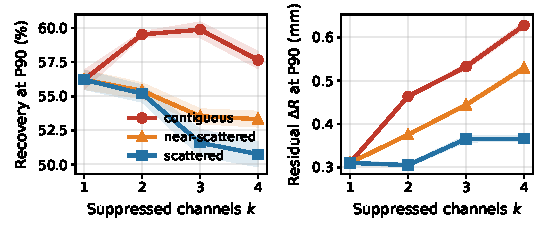
\includegraphics[width=\linewidth]{multidead_2panel}
\caption{Recovery and residual displacement as the number of simultaneously
suppressed channels grows, for the model trained on \emph{near} and
evaluated under the three failure geometries. Left, recovery at P90; right, the
displacement that remains after imputation. Lines are the mean over three
independently trained models and the shaded band their standard deviation. The
two panels show the opposite readings discussed in the text: contiguous failures
give the highest recovery and, at the same time, the largest residual error.}
\label{fig:multidead}
\end{figure}

\subsection{Physical Fidelity}
\label{sec:res-fidelity}

Recovering the position is not the same as restoring a physically admissible
signal, so we measured the two quantities the detector is built to deliver.

Separating the positioning error into its two components gives a result that a
single aggregate figure would hide (Table~\ref{tab:fidelity}). The systematic
shift falls from 0.1262\,mm to $0.0220 \pm 0.0020$\,mm, so imputation removes
$82.6 \pm 1.6$\,\% of it. The random spread, measured as the
Gaussian-equivalent FWHM of Eq.~\ref{eq:fwhm}, falls from 0.1656\,mm to
$0.0872 \pm 0.0015$\,mm, a reduction of only $47.3 \pm 0.9$\,\%
(Fig.~\ref{fig:resolucion}).

The asymmetry between the two is consistent with what the model can and cannot
know. A systematic shift is predictable from the surviving channels, because it
depends on which channel is missing and on where in the crystal the event
occurred, both of which the network sees. The random component is the part of
the lost charge that the neighbours do not determine, and no amount of
information from them recovers it. After imputation the error distribution is
therefore almost centred on the true position, and what remains is scatter
around it.

\begin{table}[t]
\centering
\caption{Components of the positioning error before and after imputation. Mean
$\pm$ standard deviation over three independently trained models; the degraded
column does not depend on the model.}
\label{tab:fidelity}
\begin{tabular}{@{}lccc@{}}
\toprule
 & \textbf{Degraded (mm)} & \textbf{Imputed (mm)} & \textbf{Removed (\%)} \\
\midrule
Systematic shift & 0.1262 & $0.0220 \pm 0.0020$ & $82.6 \pm 1.6$ \\
Random spread    & 0.1656 & $0.0872 \pm 0.0015$ & $47.3 \pm 0.9$ \\
\bottomrule
\end{tabular}
\end{table}

\begin{figure}[t]
\centering
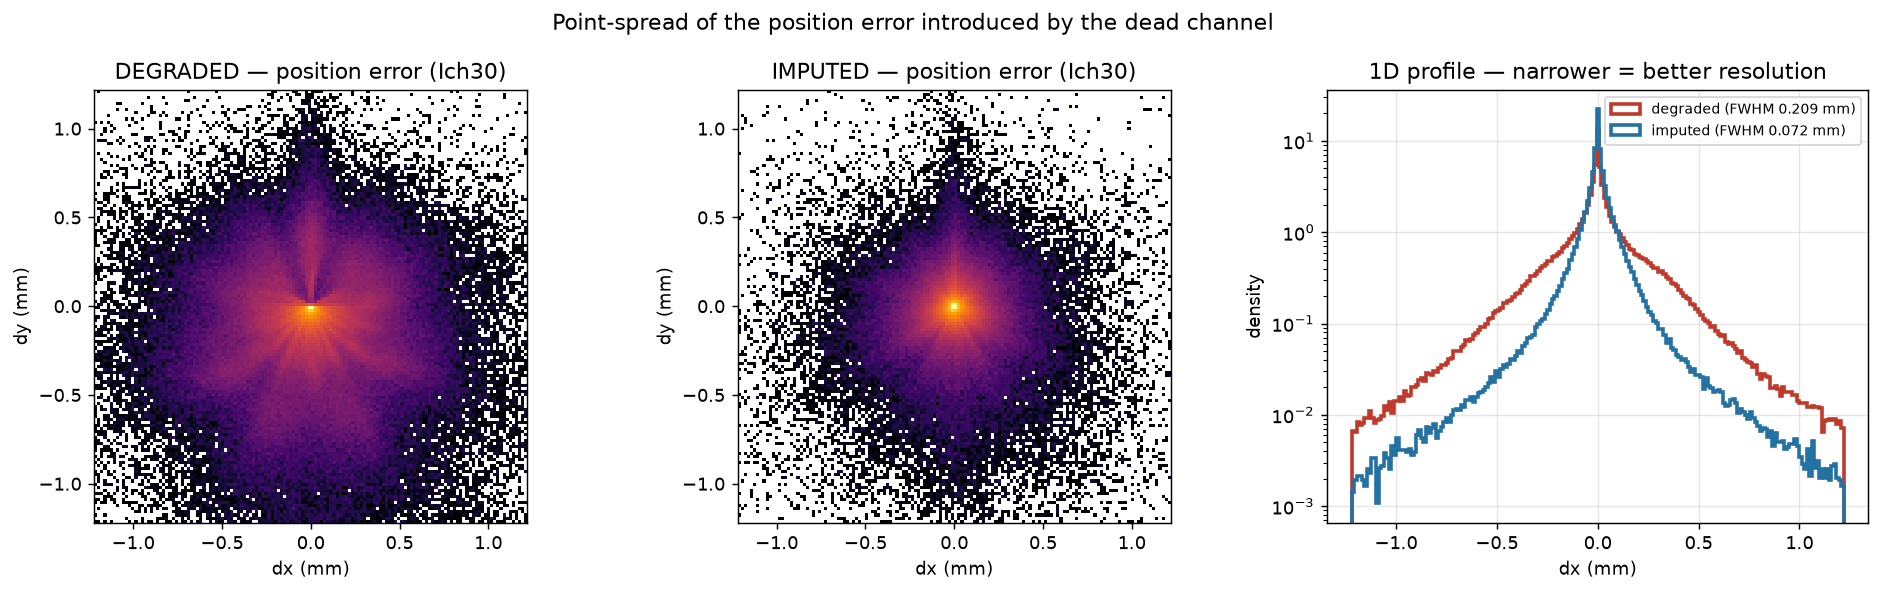
\includegraphics[width=\linewidth]{resolucion}
\caption{Distribution of the positioning error introduced by a suppressed
channel, before and after imputation. There are two conditions and not three:
the intact event is the reference against which the error is measured, so its
error is zero by construction. The width of each distribution is the quantity
reported as FWHM in Eq.~\ref{eq:fwhm}.}
\label{fig:resolucion}
\end{figure}
%v2.1Se va a experimentar con multidead para añadir estos resultados. 

The energy spectrum is preserved to a comparable degree, with a global spectral
recovery of $84.7 \pm 0.9$\,\% ($n=3$, Fig.~\ref{fig:espectro}). Here the
core-to-edge gradient reappears: $87.4 \pm 1.8$\,\% in the core,
$85.6 \pm 0.7$\,\% in the middle band and $81.2 \pm 0.3$\,\% at the edge. The
residual shift of the photopeak stays at $0.21 \pm 0.02$ ADC units across the
three zones, against the 1.6 to 1.9 ADC units that the fault introduces before
correction.

Both figures so far concern a single suppressed channel. Repeating the spectral
measurement as $k$ grows gives a result we did not expect
(Table~\ref{tab:espectro-k}): the spectrum is \emph{not} progressively lost.
Recovery goes from $83.1 \pm 0.2$\,\% with one channel to $88.7 \pm 0.3$\,\%
with four. The reason is again that recovery is a ratio. Suppressing four
channels shifts the photopeak by 4.78 ADC units instead of 1.78, and the
residual shift after imputation grows from 0.24 to 0.46, so the damage roughly
triples while what remains of it only doubles.

The three failure geometries also reorder themselves with respect to the
positioning results. At $k=4$ the contiguous geometry gives the lowest spectral
recovery, $85.6 \pm 4.8$\,\%, and the scattered one the highest,
$93.3 \pm 0.4$\,\%, which is the opposite of the ordering in
Table~\ref{tab:regimes-k}. In absolute terms, however, the two metrics agree:
contiguous failures leave the largest residual in both, 0.628\,mm of
displacement and 0.628 ADC units of photopeak shift, and scattered ones the
smallest. Compact groups remove a large amount of light from one region of the
crystal, which is hard to restore in energy, while spreading the same four
failures across the array keeps each individual deficit small. The \emph{near}
geometry sits between the two in both metrics and is the most stable of the
three, with a standard deviation of 0.3 points against the 4.8 of the
contiguous case.

\begin{table}[t]
\centering
\caption{Spectral recovery as the number of suppressed channels grows, and by
failure geometry at $k=4$. Mean $\pm$ standard deviation over three models
trained on \emph{near}. Photopeak shifts in ADC units.}
\label{tab:espectro-k}
\begin{tabular}{@{}lccc@{}}
\toprule
& \textbf{Recovery (\%)} & \textbf{Shift deg.} & \textbf{Shift imp.} \\
\midrule
$k=1$ & $83.1 \pm 0.2$ & 1.78 & 0.24 \\
$k=2$ & $87.2 \pm 0.8$ & 2.80 & 0.34 \\
$k=3$ & $90.1 \pm 1.7$ & 3.88 & 0.33 \\
$k=4$ & $88.7 \pm 0.3$ & 4.78 & 0.46 \\
\midrule
$k=4$, cluster & $85.6 \pm 4.8$ & 5.03 & 0.63 \\
$k=4$, near    & $88.7 \pm 0.3$ & 4.78 & 0.46 \\
$k=4$, scatter & $93.3 \pm 0.4$ & 3.62 & 0.20 \\
\bottomrule
\end{tabular}
\end{table}

%v2.1 Esta grafica es compacta pero uff, igual la que enseña los espectros por zonas es más cuca y se ve el del Na22.  [Checked]
% Cambiada por espectros_zonas, que ensena los histogramas de verdad en vez del
% resumen agregado. A doble columna, que con quince paneles no cabe en una.
\begin{figure*}[t]
\centering
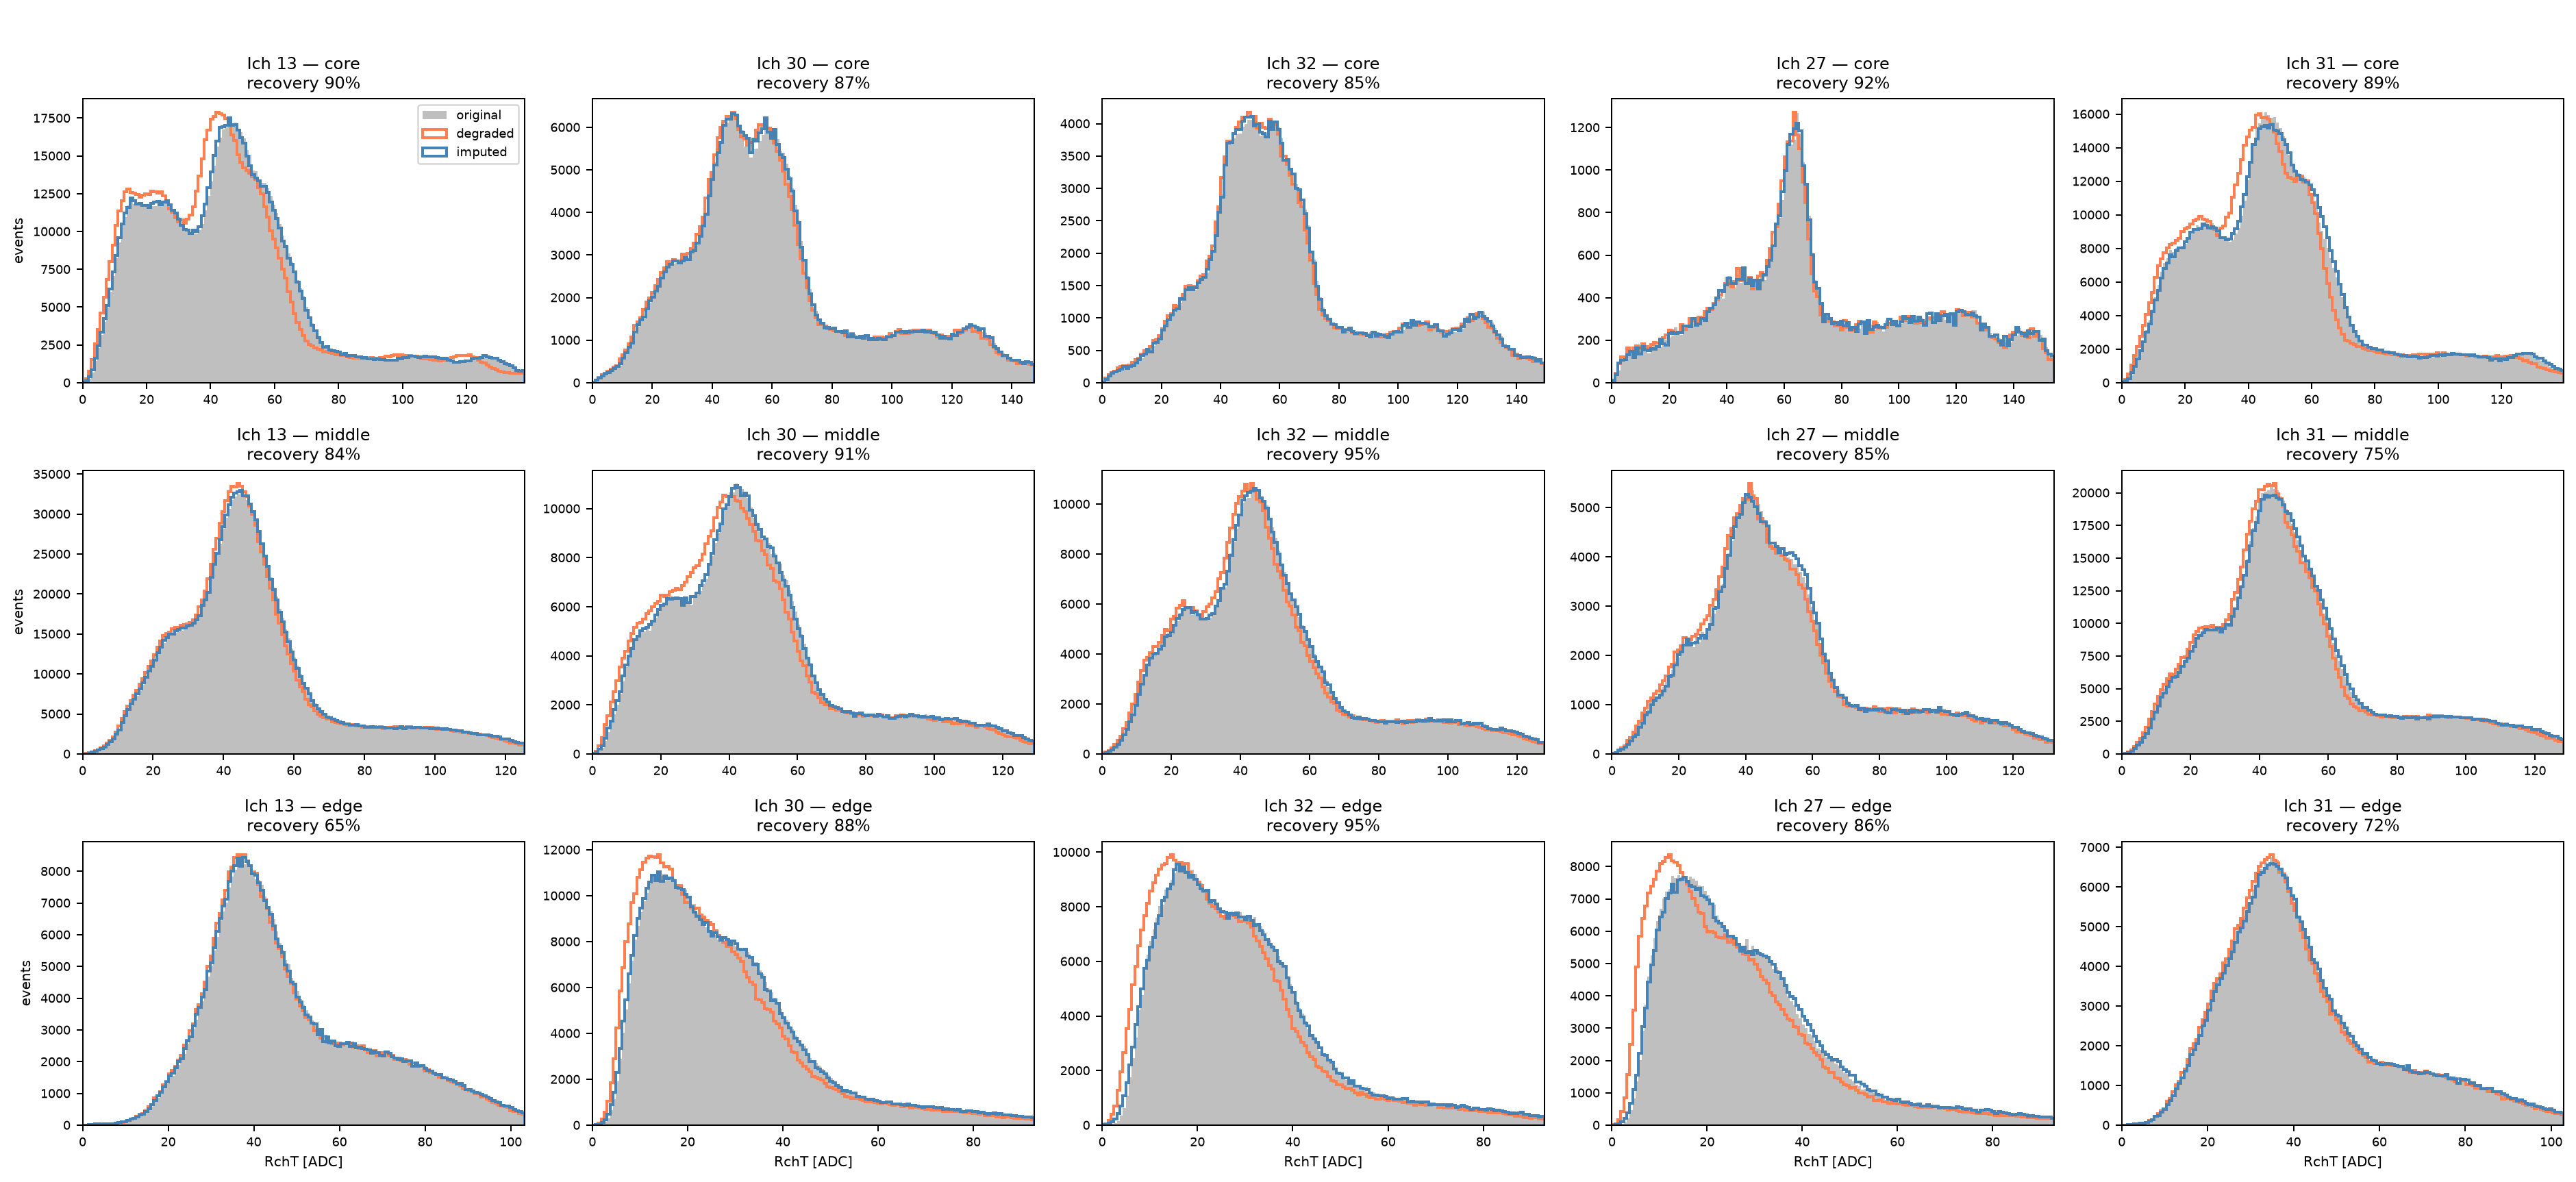
\includegraphics[width=\textwidth]{espectros_zonas}
\caption{Energy spectra of the affected events for five channels (columns) and
the three crystal zones (rows), comparing the original distribution in grey with
the degraded one in orange and the imputed one in blue. The 511\,keV photopeak
of $^{22}$Na is visible in the core and middle rows and flattens towards the
edge, where the absorbing adhesive removes part of the collected light. The
degraded curve departs from the original towards lower energies, and imputation
brings it back; the per-panel figure is the spectral recovery.}
\label{fig:espectro}
\end{figure*}

\subsection{Variants That Did Not Improve the Model}
\label{sec:res-negative}

%v2.1Muy cutres estas secciones, hay que añadir ecuaciones, ya que en materiales y metodos apenas se dicen en 2 frases, si se ha usado se debe de desarrollar.  [Checked]
%v2.1 De nuevo, ecuaciones, parametros, etc... [Checked]
%v2.1 Que ensembles se hicieron,etc... [Checked]
Four of the alternatives outlined in Sections~\ref{sec:arch} and
\ref{sec:training} failed to improve on the reference. We report them with the
form each one took, because in three of the four the reason for the failure lies
in that form rather than in the idea behind it.

\subsubsection{Physics-informed terms}
Both variants add a penalty to the loss of Eq.~\ref{eq:loss},
%
\begin{equation}
\mathrm{Loss} = \mathrm{Loss}_{\mathrm{MSE}} + \lambda \, \Phi,
\label{eq:physloss}
\end{equation}
%
with $\Phi$ the physical quantity to preserve. We calibrated $\lambda$ in each
case so that both terms contribute comparably at the start of training.

The first uses the squared displacement of the centroid,
$\Phi_{\Delta R} = \Delta R^{2}$ with $\lambda = 0.01$, computed with the same
charge-weighted centroid as the evaluation metric. It changes recovery from
58.0\,\% to 58.2\,\%, inside the run-to-run band. The term turns out to be
largely redundant: for a given channel, charge and position are related
monotonically, so penalising the position error adds little that the MSE on the
charge was not already penalising.

The second targets the energy spectrum, $\Phi_{E} = \lvert \Delta R_{T} \rvert$
with $\lambda = 0.7$, where $\Delta R_{T}$ is the shift in mean total charge.
This one is actively harmful: recovery falls to 46.0\,\% and the bias changes
sign. The cause is the form of the term and not the quantity it targets. The
shift is computed over a batch, so the penalty acts on a \emph{signed average}
and the model can reduce it by letting errors of opposite sign cancel between
events. It optimises the aggregate while degrading every individual event, which
is exactly what the per-event metrics detect. A physics-informed term for this
problem has to be computed per event.

\subsubsection{Heteroscedastic prediction}
Here the network outputs a mean and a log-variance per channel and trains on the
Gaussian negative log-likelihood,
%
\begin{equation}
\mathrm{Loss}_{\mathrm{NLL}} = \frac{(y_{c} - \mu_{c})^{2}}{2\sigma_{c}^{2}}
                             + \log \sigma_{c},
\label{eq:nll}
\end{equation}
%
which would let the model flag the events it cannot impute reliably. It reaches
20.1\,\%. The likelihood offers two ways of lowering the loss, improving $\mu$
or inflating $\sigma$, and with nothing tying $\sigma$ to a calibration target
the second is cheaper. The model learns to declare uncertainty instead of
learning to predict.

\subsubsection{Ensembles}
Averaging the outputs of several models is the only variant that exceeds the
reference band, and it does so modestly. We tested two compositions. The first
averages three replicas of the reference, identical except for the random seed,
and reaches 58.69\,\%. The second averages three different architectures ---
\textsc{HexGNN} with isotropic mean aggregation, PNA with multiple aggregators
and a directional hexagonal convolution --- on the assumption that their errors
would be less correlated, and reaches 58.73\,\%. Against $58.04 \pm 0.37$\,\%
for a single model, both gain about 0.7 points, and the heterogeneous
composition adds almost nothing over the homogeneous one. The cost is three
forward passes per event.


% ---------------------------------------------------------------------
\section{Discussion}
\label{sec:discussion}
% ---------------------------------------------------------------------

\subsection{What the Method Achieves}

The question posed in Section~1 was whether the signal of a failed channel can
be reconstructed instead of discarded. It can. On detectors the network has
never seen, imputation removes $56.6 \pm 2.3$\,\% of the positioning error that
the fault introduces, leaving a residual displacement of 0.28\,mm at P90 --- a
7.5\,\% of the distance between neighbouring sensors. The energy spectrum
survives the operation at $84.7 \pm 0.9$\,\%, with a photopeak displaced by
0.21 ADC units where the uncorrected fault displaces it by 1.8.

Two properties of the approach matter as much as those numbers. The supervision
is generated from healthy modules, so no detector with a genuinely dead sensor
is needed to train, and the correction is applied before the centre of gravity
is computed, so it returns a complete 61-channel vector that any downstream
stage consumes unchanged.

\subsection{Why a Small Network Suffices}

The result that most constrains the interpretation is that a graph network of
\num{38305} parameters matches or exceeds every alternative we tried, including
a graph transformer with a hundred times more parameters. This is not evidence
that attention mechanisms are ineffective in general; it is evidence about the
problem. The information that determines the charge of a missing channel is
concentrated in its immediate surroundings, and once a model has access to it,
additional capacity has nothing further to extract.

Three independent measurements support that reading. Restricting the linear
baselines to concentric rings shows that the second ring already captures
essentially everything: the third adds 0.09 points and the remaining 47
channels a further 0.04. Architectures with a wider receptive field perform
three points worse rather than better, which is what one expects when the extra
context is mostly noise. And permuting the adjacency while preserving the
degree distribution collapses recovery from 58 to 28\,\%, so what the model
exploits is the specific geometry of the detector and not the inductive bias of
message passing.

This is consistent with the physics. Light sharing in a monolithic crystal is a
local phenomenon: the charge collected by a sensor is determined by the
interactions that occur near it, and the redundancy that makes imputation
possible lives in that neighbourhood.

%v2.2 Esta seccion no me gusta mucho creo que es mejor comentar que el problema real es complejo
% y faltan calibraciones, datos reales y poder parear un GT que nos limitan los resultados.
%Esta muy escueto y creo que es lo mas importante de comentar no?  Todo esto me pega mas en limitaciones
% [Checked] Reescrita entera. Antes respondia "que limita el rendimiento" solo
% con la variabilidad entre modulos, que es un sintoma. Ahora responde con la
% causa: son datos reales, sin calibrar y sin referencia posible para un fallo
% real. Limitations se ha recortado en paralelo para no repetirlo.
\subsection{What Limits Performance}
\label{sec:disc-limits}

If capacity is not the constraint, the natural question is what is. Our
measurements point away from the model and towards the data. Nine architectural
variants, a doubled training budget and a larger parameter count all leave
recovery within a point of the reference. What does move it, and by far, is
which detector the model is measured on: recovery ranges from 29 to 63\,\%
across individual modules, with a standard deviation of 7.9 points, against 0.3
between training runs on the same partition.

That spread is a property of the hardware, not of the method, and it is the
price of working with real acquisitions. The 159 modules were built and
assembled one by one, and they differ in ways the network never observes: the
gain of each individual photosensor, the quality of the optical coupling
between crystal and array, the exact placement of the source during each
acquisition. No energy calibration was applied, so the charge the model reads
is in ADC units whose scale is not common to all modules. A model trained
across the ensemble can only learn what the ensemble shares; whatever is
specific to one detector is, by construction, outside its reach.

There is a second consequence of using real data, and it bounds what can be
verified rather than what can be learned. The fault we inject is synthetic
because a real one leaves no reference: on a module whose channel is genuinely
dead there is no way to know what that channel should have read, and therefore
no way to measure the error of the imputation. Everything reported here is
measured on healthy hardware with a fault we created, and the agreement between
that setting and a real failure is an assumption, not a measurement. It is a
reasonable assumption --- the mask reproduces patterns we observed in the 62
defective modules --- but it is worth stating as one.

Read together, the two points set the terms in which any figure in this work
should be taken. Comparisons between models are precise, because they are
paired over the same modules, events and masks. The absolute value on a new
detector carries the variability of the hardware, and the way to reduce it is a
per-module calibration rather than a better network.

%Efectivamente creo que es muy largo. [Checked: de cuatro parrafos a dos]
\subsection{Behaviour Under Multiple Failures}

Training on single failures does not transfer to multiple ones, and the gap,
24.6 points, is the largest effect we measured. The geometry used to build the
training masks matters far less: training on \emph{near} gains 1.99 points on
its own terrain and is indistinguishable from \emph{cluster} elsewhere. The
practical recommendation is therefore simpler than we expected --- train with
one to four channels suppressed and do not worry much about the pattern.

Two things about the energy did surprise us. The spectrum does not degrade as
failures accumulate: recovery rises from 83 to 89\,\% between one and four
suppressed channels, because the metric is a ratio and the damage grows faster
than the residual. And the three geometries reorder themselves with respect to
the positioning results, contiguous failures being the easiest case in position
and the hardest in energy. A compact group displaces the centroid greatly but
predictably, since the ring of surviving sensors around it still describes
where the light went, while removing that much charge from one region is what
makes the energy hard to restore. In absolute terms both metrics agree that a
contiguous group is the worst case; it is only as a ratio that they disagree.
The practical reading is that the energy information degrades gracefully, which
is what a downstream energy window needs.

\subsection{Relation to Existing Practice}

Industrial quality control identifies dead pixels and compensates for them
downstream, either by duplicating events from neighbouring pixels in list mode
or by interpolating in sinogram space \cite{philips2015deadpixel}. The channel
itself is never recovered. The approach taken here intervenes earlier, before
the centre of gravity is computed, and therefore preserves the crystal
identification that downstream compensation cannot restore.

It also differs from the deep learning work closest to it. Networks trained to
invert multiplexed readout schemes reconstruct individual channel values from a
reduced set of measurements \cite{li2023, niu_cnn-based_2024}, and the approach
extends to semi-monolithic detectors where the full response is recovered from
row and column sums \cite{loignon-houle_multi-input_2026}. In all of those
cases the information is present in the acquired data, encoded in a linear
combination fixed by design, and the network learns to invert a known mapping.
A failed channel is a different problem: nothing of its signal reaches the
acquisition, and the only remaining trace is the statistical correlation that
light sharing induces among its neighbours.

% [Checked] Anadido el parrafo sobre el encaje con Jimenez Algarra e
% Hidalgo-Torres, sin comparar cifras -no son comparables- y llevandolo hacia
% la ventaja del monolitico, como pediste.
That last point is what connects this work with the other deep learning studies
on this same detector. Both estimate the interaction position from the 61
channels, one on simulated data \cite{jimenez2025} and one on measured
\cite{hidalgo2022, hidalgo-torres_predicting_2020}. Ours does not compete with
them: it repairs the 61-channel vector that they take as input, and the two are
consecutive stages of the same chain. What they have in common is more
interesting than what separates them. All three exploit the fact that in a
monolithic crystal the light of one event reaches many sensors, so the array
carries more information than the number of channels suggests --- position
between sensors in their case, the value of a missing sensor in ours. A
pixelated detector offers neither: its segmentation fixes the spatial
resolution at the pixel pitch, and a dead pixel is a hole with no redundancy to
fill it from. That redundancy is difficult to exploit analytically, which is
historically why monolithic designs were set aside, and it is exactly what a
learned model is good at. The results reported here suggest that this is also
where their remaining margin lies.

\subsection{Limitations}

Three limitations bound what the preceding results support, beyond the two
properties of the data discussed in Section~\ref{sec:discussion}.

The test partition contains five modules. Given the variability between
detectors, that places the standard error of any absolute figure at
approximately 3.5 points, which is why we report cross-validated values rather
than the result of a single partition.

The simulated fault is a total suppression. Real degradation is often partial:
a channel that keeps part of its response, or that drifts with temperature. The
method has not been evaluated in that regime, and it is not obvious that a
model trained on complete failures transfers to it.

%v.2.2 Si que sabemos, es por la variabilidad de los datos reales, no son simulaciones,
% hay datos que tienen menos info sobre un canal por azar, porque ese canal puede tener
% algo menos de ganancia, por posicionamiento del emisor, osea no creo que sea correcto
% decir eso simplemente comentar que en lineas futuras un trabajo con datos simulados o
% ultracontrolados permitira analizar esto mejor. [Checked]
Finally, the minimum over the 61 channels proved unusable as a robustness
metric, and the reason is instructive rather than mysterious. Its variation
across training runs, $\pm 4.5$ points, exceeds any difference we could have
attributed to a design choice, and the channel attaining it changes from run to
run. A minimum over 61 values is a noisy statistic to begin with, and here it
lands on whichever channel happens to be worst served by the data: the sensors
do not all have the same gain, the source was not equidistant from all of them,
and some channels simply receive less usable light than others in a given
acquisition. What the metric measures is therefore closer to the luck of the
acquisition than to the robustness of the model. Separating the two would
require data in which the per-channel response is known or controlled, which
real flood acquisitions do not provide.

%v2.2 comentar lo que te digo arriba aqui mas extenso, no ser tremendista si no decir que
% hemos sentado unas bases en este campo y que estas son las lineas futuras. Aunque ahora
% que lo pienso esto queda mejor en la conclusion.
% [Checked] Ampliada y en tono de lineas abiertas, no de deficiencias. El "hemos
% sentado unas bases" NO se dice aqui a proposito: si va tambien en Conclusions
% suena a autobombo repetido. Lo dejo para que lo digas tu una sola vez alli.
\subsection{Future Work}

Four directions follow from the above, and the first two address the two
limits identified in Section~\ref{sec:discussion} rather than any shortcoming of
the network.

A calibrated acquisition would separate what belongs to the method from what
belongs to the hardware. With per-channel gains known, the charge of every
module would live on a common scale, the spectral metric could be reported in
keV instead of as a conservation ratio, and the spread between detectors could
be attributed rather than merely measured. A complementary route is a
controlled simulation of this same geometry, where the response of each sensor
is set rather than inferred: it would make the worst-channel behaviour
analysable, and it would allow the synthetic fault to be validated against a
known reference.

The second is the 62 modules with genuine defects, of which 18 are annotated so
far. They cannot give a quantitative error, for the reason given above, but
they can answer a question the synthetic experiments cannot: whether an
imputation trained on injected faults produces flood maps that an expert
accepts as repaired.

The third is partial degradation. Extending the training masks to channels that
keep part of their response, rather than none of it, would cover the failure
mode that the current model does not see and that the annotation campaign
suggests is the more common one in practice.

The fourth concerns what the imputation is for. Everything here is measured on
single detectors, and the quantity that matters clinically is the resolution of
the reconstructed image. Propagating imputed events through a full
reconstruction, and quantifying what a repaired module contributes to a ring of
them, is the step that would turn a per-detector correction into a
system-level result.


% ---------------------------------------------------------------------
\section{Conclusions}
\label{sec:conclusions}
% ---------------------------------------------------------------------
% Adaptado del boceto de Miguel (v2.2). Cambios de fondo respecto a ese
% boceto, todos por coherencia con lo que el paper ya afirma:
%   - "58 % en el mejor de los casos" -> 56,6 +/- 2,3. La 3.4 cierra
%     explicitamente que 56,56 +/- 2,32 es la cifra para hardware no visto;
%     dar 58 aqui contradice esa seccion.
%   - Fuera la reduccion de dosis y de tiempo de adquisicion: no se ha
%     medido ninguna de las dos. Queda la idea que si se sostiene, que es
%     no tirar informacion ya adquirida.
%   - "como se reviso en los datos reales" -> los 62 modulos defectuosos se
%     INSPECCIONARON para sacar los patrones; la evaluacion es sintetica.
%     La 4.3 dice justo eso dos paginas antes.
%   - Cristal monolitico = centelleador, no fotomultiplicador.
%   - Anadido el espectro (84,7 %) y la autosupervision, que el boceto no
%     mencionaba y son la mitad del resultado.

We have presented a deep learning method that recovers the signal lost to a
faulty SiPM channel in a monolithic PET detector instead of discarding it.
Monolithic scintillators are cheaper to produce than pixelated arrays and they
do not impose a segmentation on the information that reaches the reconstruction
stage, but they pay for it with a readout in which every sensor contributes to
every event: when one channel fails, the flood map degrades across the whole
crystal and the module is normally set aside. Recovering that channel is
therefore a way of keeping detectors, and the events they have already
acquired, that current practice gives up.

The method is a graph neural network, \textsc{HexGNN}, built on the geometry of
the array rather than on top of it: one node per sensor, one edge between
adjacent sensors, and message passing along the same paths through which the
light is shared. It has \num{38305} parameters. Its supervision comes from
healthy modules --- we suppress a channel whose true value we know --- so no
detector with a genuine fault is needed in order to train it, and the
correction is applied before the centre of gravity is computed, which returns a
complete 61-channel vector that the rest of the processing chain consumes
unchanged.

On modules the network had never seen, imputation removes $56.6 \pm 2.3$\,\% of
the positioning error introduced by the fault, leaving a residual displacement
of 0.28\,mm at P90, and it preserves the energy spectrum to
$84.7 \pm 0.9$\,\%. Training with one to four simultaneous failures, following
the patterns we found in the flood maps of the modules that arrived with a
defect, extends that behaviour to several dead channels at no cost in the
single-channel case.

Industrial practice discards the faulty channel, so there was no figure to
improve on: the one reported here is a first reference for a problem nobody had
addressed upstream of the centroid. Three lines follow from it --- a calibrated
acquisition, which would separate what belongs to the method from what belongs
to the hardware; the modules that arrived with a defect, which offer a
validation against expert criterion that no injected fault can give; and a full
reconstruction of imputed events, which would take the correction from the
detector to the system. What the work establishes is that the information
needed to repair a dead channel is there in its neighbours, and that a small
network with the geometry of the detector built into it is enough to reach it.


% ---------------------------------------------------------------------
% REFERENCIAS
% ---------------------------------------------------------------------
\bibliographystyle{IEEEtran}
\bibliography{referencias}

\end{document}